\documentclass[conference,a4paper]{IEEEtran}
\IEEEoverridecommandlockouts
\usepackage[utf8]{inputenc}
\usepackage[T1]{fontenc}
\usepackage[spanish,es-noshorthands,es-tabla]{babel}
\usepackage{cite}
\usepackage{amsmath,amssymb}
\usepackage{graphicx}
\usepackage{booktabs}
\usepackage{tikz}
\usetikzlibrary{arrows.meta,positioning}
\usepackage[hidelinks]{hyperref}
\usepackage{xurl}
\graphicspath{{figures/}{../../figuras/01_articulos_eda/}{../../figuras/02_articulos_clustering_reglas/}{../../figuras/03_imu_perfiles/}{../../figuras/04_ml_clasificacion/}{../../figuras/05_catalogo_datasets/}{../../figuras/06_regresion/}{../../figuras/07_cloud_aws/}}
\renewcommand{\IEEEkeywordsname}{Palabras clave}

% Inserta la captura si existe; si no, deja un recuadro con su nombre
\newcommand{\captura}[2]{\IfFileExists{capturas/#1}{\includegraphics[width=#2]{capturas/#1}}{\IfFileExists{../../figuras/07_cloud_aws/capturas/#1}{\includegraphics[width=#2]{../../figuras/07_cloud_aws/capturas/#1}}{\fbox{\parbox[c][2.2cm][c]{0.95#2}{\centering\small Captura pendiente: \detokenize{#1}}}}}}

\usepackage{float}
\usepackage[section]{placeins}
\begin{document}

\title{Detección de cojera equina mediante minería de datos, aprendizaje automático y computación en la nube}

\author{\IEEEauthorblockN{Carlos Josué Barrera Vargas}
\IEEEauthorblockA{Facultad de Ingeniería de Datos e Inteligencia Artificial\\
Universidad Santo Tomás, Seccional Tunja, Colombia\\
Proyecto integrador de quinto semestre · Minería de Datos, Machine Learning y Cloud Computing\\
Repositorio: \url{https://github.com/Cjoh210/Proyecto_Deteccion_Marcha_Equina}}}

\maketitle

\begin{abstract}
La cojera acostumbra ser el problema de salud más común en caballos, el problema es que su diagnóstico depende totalmente en una evaluación subjetiva. Este trabajo concentra la fase exploratoria de un sistema para detectarla de manera objetiva, así mismo tiene la intención de trabajar en etapas futuras con video. Se siguió la metodología CRISP-DM para procesamiento de información usando artículos científicos, un catálogo de datasets abiertos y señales de sensores de 22 caballos con cojera inducida. El proceso de minería de datos mostró que el campo se proyecta al uso de visión por computadora, por otro lado una falta de investigación en Colombia y de datasets que contengan video y cojera natural. El análisis de señales confirmaron que una asimetría en el movimiento de la cabeza y pelvis del sujeto delatan cojera, demostrado en un modelo validado con datos nuevos para probar generalización. Este sistema completo fue desplegado en AWS usando Terraform, con una arquitectura serverless.
\end{abstract}

\begin{IEEEkeywords}
minería de datos, CRISP-DM, aprendizaje por ensambles, computación en la nube, cojera equina, desarrollo sostenible
\end{IEEEkeywords}

\section{Introducción}

La cojera en los caballos suele ser el primer indicio del deterioro de la salud y una condición ciertamente costosa para el sector, porque se pierde tiempo de uso del animal al requerir reposo y la necesidad de un tratamiento largo y laborioso~\cite{nehs2013,usda1998}. El diagnóstico se basa sobre todo en observar al animal al trote, y varios estudios muestran que los veterinarios coinciden poco entre sí cuando se presenta una cojera leve~\cite{keegan2010,hammarberg2016}.

En Colombia hay cerca de un millón de equinos registrados~\cite{agronegocios2025censo}, y el caballo criollo tiene un valor cultural y económico importante en regiones como los llanos Orientales y Boyacá. Un sistema que estime la cojera a partir de un video del celular establecería un estándar técnico de evaluación del que veterinarios de campo y criadores pueden beneficiarse. Antes de construirlo, este trabajo responde tres preguntas: qué se ha investigado y dónde está el vacío, con qué datos públicos se cuenta y qué señales del movimiento delatan a un caballo cojo. Con esas respuestas se construyó un modelo predictivo y se desplegó en la nube como un servicio completo.

\section{Planteamiento del problema}

La evaluación de la cojera es subjetiva, y los métodos objetivos, como sensores corporales, plataformas de fuerza o captura de movimiento, son costosos o exigen instrumentar al animal. Por eso quedan fuera del alcance de muchos criadores y veterinarios rurales.

\textbf{Pregunta de investigación.} ¿Es posible estimar la probabilidad de que un caballo esté cojo a partir de datos de movimiento obtenibles con tecnología accesible, de forma interpretable y con bajo costo de despliegue?

\textbf{Usuarios y beneficiarios.} Veterinarios de campo, que ganan una segunda opinión objetiva y un seguimiento en el tiempo; criadores y asociaciones de caballo criollo, que pueden vigilar a sus animales; y los propios caballos, que reciben un diagnóstico más temprano.

\textbf{Alineación con los ODS.} El proyecto se vincula con el ODS 3, Salud y bienestar, desde el enfoque de Una Salud, que integra la salud animal y humana~\cite{un2015}, y con el ODS 8, Trabajo decente y crecimiento económico, al reducir pérdidas en un sector rural que genera empleo.

\section{Trabajo relacionado}

La evaluación objetiva de la cojera se ha apoyado en sensores inerciales en la cabeza y la pelvis, que miden cuán desigual es el desplazamiento vertical en cada paso; estas medidas se relacionan con el examen clínico, aunque no lo reemplazan~\cite{keegan2013}. En visión por computador, DeepLabCut permitió ubicar puntos anatómicos en video sin marcadores~\cite{mathis2018}, y aparecieron datasets de caballos como Horse-10 y PFERD~\cite{mathis2021,li2024pferd}, junto con bancos de pose de muchas especies como AP-10K, APT-36K y Animal Kingdom~\cite{yu2021ap10k,yang2022apt36k,ng2022animalkingdom}. Ninguno incluye etiquetas clínicas de cojera. La detección automática está más avanzada en bovinos, con bases públicas como CowScreeningDB~\cite{ismail2024cow}. Este trabajo cuantifica ese vacío y propone una forma de cerrarlo.

\section{Marco teórico}

El trabajo combina técnicas de minería de datos, aprendizaje automático y computación en la nube. Esta sección resume las que sostienen los resultados principales.

\subsection{Conceptos y siglas}

\begin{itemize}
\item \textbf{CRISP-DM:} metodología estándar de minería de datos con seis fases, de comprensión del problema al despliegue~\cite{wirth2000}.
\item \textbf{EDA:} análisis exploratorio de datos con revisión inicial de estadísticas y gráficas.
\item \textbf{IQR:} rango intercuartílico, es decir, distancia entre el primer y el tercer cuartil.
\item \textbf{PCA:} análisis de componentes principales para conservar varianza.
\item \textbf{SVD:} descomposición en valores singulares, reducción de dimensionalidad de matrices.
\item \textbf{DBSCAN:} algoritmo de agrupamiento basado en densidad que marca los puntos aislados como ruido.
\item \textbf{Apriori y FP-Growth:} algoritmos que encuentran elementos que aparecen juntos con frecuencia y generan reglas de asociación~\cite{agrawal1994,han2000}.
\item \textbf{KNN:} clasificador para asignar la clase de los casos más cercanos.
\item \textbf{SVM:} clasificador para separar clases con la frontera de mayor margen.
\item \textbf{Validación cruzada:} evaluación de un modelo en varias particiones distintas de los datos.
\item \textbf{Grid Search y Random Search:} búsqueda de hiperparámetros.
\item \textbf{ROC-AUC:} mide la capacidad del modelo para separar las clases, de 0,5, igual al azar, a 1, perfecta.
\item \textbf{API:} interfaz que permite a otro programa enviar datos al sistema y recibir una respuesta.
\item \textbf{ODS:} Objetivos de Desarrollo Sostenible de las Naciones Unidas~\cite{un2015}.
\end{itemize}

\subsection{Asimetría de la marcha}

Al trote, la cabeza y la pelvis suben y bajan dos veces por zancada. En un caballo sano ambas partes son casi iguales; cuando una pata le duele, el animal descarga peso y el movimiento se vuelve asimétrico~\cite{keegan2013}. Se mide con la diferencia entre los dos puntos más bajos y entre los dos más altos del desplazamiento vertical en cada zancada:

\begin{gather*}
\mathrm{MinDiff} = z_{\min,1} - z_{\min,2} \\
\mathrm{MaxDiff} = z_{\max,1} - z_{\max,2}
\end{gather*}

\subsection{Representación y agrupamiento}

Cada resumen se convierte en un vector con TF-IDF, que da peso a los términos frecuentes en un documento~\cite{salton1988}:

\[
\mathrm{tfidf}(t,d) = \mathrm{tf}(t,d)\cdot \log\frac{N}{\mathrm{df}(t)}
\]

La matriz se reduce con SVD y se agrupa con K-Means, que busca los k centros que minimizan la distancia de cada punto a su grupo~\cite{lloyd1982}. Para el catálogo de datasets, con variables numéricas y categóricas mezcladas, se usa la distancia de Gower, que promedia una diferencia normalizada por variable~\cite{gower1971}. Los atípicos son detectados con Isolation Forest, que aísla los puntos con cortes al azar en el muestrario~\cite{liu2008}.

\subsection{Ensambles e interpretabilidad}

Random Forest promedia muchos árboles entrenados con muestras y variables distintas, de manera que reduce la varianza~\cite{breiman2001}; Gradient Boosting añade árboles en las iteraciones para corregir el error del anterior~\cite{friedman2001}, y para explicar las predicciones se usa \textbf{SHAP}, que reparte las predicciones entre las variables según el aporte marginal promedio~\cite{lundberg2017}:

\[
\phi_i = \sum_{S \subseteq F \setminus \{i\}} \frac{|S|!\,(|F|-|S|-1)!}{|F|!}\,\big[f(S \cup \{i\}) - f(S)\big]
\]

\subsection{Regresión regularizada}

La regularización penaliza los coeficientes grandes para evitar el sobreajuste. Elastic Net~\cite{zou2005} combina la penalización de Lasso, que lleva coeficientes a cero y selecciona variables~\cite{tibshirani1996}, con la de Ridge; con $\alpha$ = 1 se obtiene Lasso y con $\alpha$ = 0, Ridge:

\[
\min_{\beta}\; \lVert y - X\beta \rVert^2 + \lambda \big[ \alpha \lVert\beta\rVert_1 + (1-\alpha) \lVert\beta\rVert_2^2 \big]
\]

\subsection{Computación sin servidores}

La nube ofrece recursos bajo demanda en distintos modelos de servicio: IaaS, PaaS y SaaS~\cite{mell2011}. En el modelo sin servidores, el código se ejecuta como funciones que se activan con el evento además de que escalan solas y se cobran por ejecución~\cite{terraform}.

\section{Sistema propuesto}

La Fig. 1 muestra el sistema completo. Las tres fuentes van a un data lake en la nube, siguen con un pipeline de minería que prepara y analiza los datos, luego un modelo aprende a reconocer la cojera a partir de medidas de simetría de la marcha sacadas; y una API entrega las predicciones y mantiene un historial para hacer el seguimiento.

\begin{figure}[!htb]
\centering
\begin{tikzpicture}[node distance=3mm and 4mm, font=\scriptsize,
  b/.style={draw, rounded corners=2pt, align=center, minimum height=7mm, text width=17mm, fill=#1!12},
  b/.default=blue, >={Stealth[length=1.6mm]}]
\node[b=orange] (api) {Artículos\\científicos};
\node[b=orange, below=of api] (cat) {Catálogo de\\datasets};
\node[b=orange, below=of cat] (imu) {Señales de\\sensores};
\node[b=gray, below=of imu] (vid) {Video móvil\\(fase futura)};
\node[b=green, right=6mm of cat, yshift=-5mm, text width=14mm, minimum height=22mm] (lake) {Data lake\\en la nube};
\node[b, right=6mm of lake, yshift=10mm] (kdd) {Minería\\de datos};
\node[b, below=of kdd] (ml) {Modelo de\\aprendizaje\\automático};
\node[b=gray, below=of ml] (cv) {Visión por\\computador};
\node[b=purple, right=4mm of ml, text width=13mm] (srv) {API y\\registro de\\predicciones};
\draw[->] (api) -- (lake); \draw[->] (cat) -- (lake); \draw[->] (imu) -- (lake);
\draw[->, dashed] (vid.east) -- ++(2mm,0) |- (cv.west);
\draw[->] (lake) -- (kdd); \draw[->] (kdd) -- (ml); \draw[->, dashed] (cv) -- (ml); \draw[->] (ml) -- (srv);
\end{tikzpicture}
\caption{Estructura general del sistema.}
\label{fig:sistema}
\end{figure}

\section{Metodología}

La metodología sigue las fases de CRISP-DM~\cite{wirth2000} y se implementó en seis notebooks. Esta sección describe cómo se obtuvieron, prepararon y exploraron los datos.

\subsection{Adquisición}

\textbf{Web scraping del estado del arte.} Un script de Python consultó la API de OpenAlex~\cite{priem2022openalex} con cinco búsquedas temáticas: cojera equina, marcha equina, sensores, visión y pose animal, y cojera con aprendizaje automático en otras especies para así construir y mantener actualizados los recursos del proyecto, con esto, se reunieron 6.472 registros.

\textbf{Catálogo de datasets.} Se documentaron catorce datasets públicos con sus características y el enlace de origen de cada uno.

\textbf{Señales de sensores.} Se descargó un dataset abierto con 22 caballos islandeses medidos sanos y con una cojera leve inducida en una extremidad anterior o posterior, registrados con dieciséis sensores inerciales~\cite{smit2023dataset}.

\subsection{Preparación}

En el corpus se fusionaron los artículos repetidos entre búsquedas y también se descartaron documentos no científicos o que no tenían que ver. Quedaron después de la limpieza 4.024 artículos.

\subsection{Ingeniería de características}

Las señales crudas de los sensores, mantenían escalas de millones de muestras que en sí mismas mostraron no ser útiles. Se tomaron las capturas de trote en línea recta, se calculó el desplazamiento vertical de la cabeza, la cruz, el sacro y las caderas, y se dividió la marcha en zancadas con el propósito de estandarizar medidas. De cada zancada se extrajeron medidas que mostraran resultados clínicos reales, de tal manera que quedaron estas variables: la diferencia entre los dos puntos más bajos y los dos más altos de cada ciclo, el rango de movimiento, la regularidad del ritmo y la diferencia entre caderas. De resultado quedó una tabla de 1.817 zancadas con 27 variables. Los faltantes que hubieran se imputaron con la mediana del mismo caballo y se eliminaron las pocas zancadas físicamente imposibles. Sobre esta tabla se aplicó PCA, donde fue evidente que varias medidas son redundantes y que las zancadas sanas y cojas se superponen en una medida considerable, esto anticipa dificultades en el proceso (Fig. 2).

\begin{figure}[!htb]
\centering
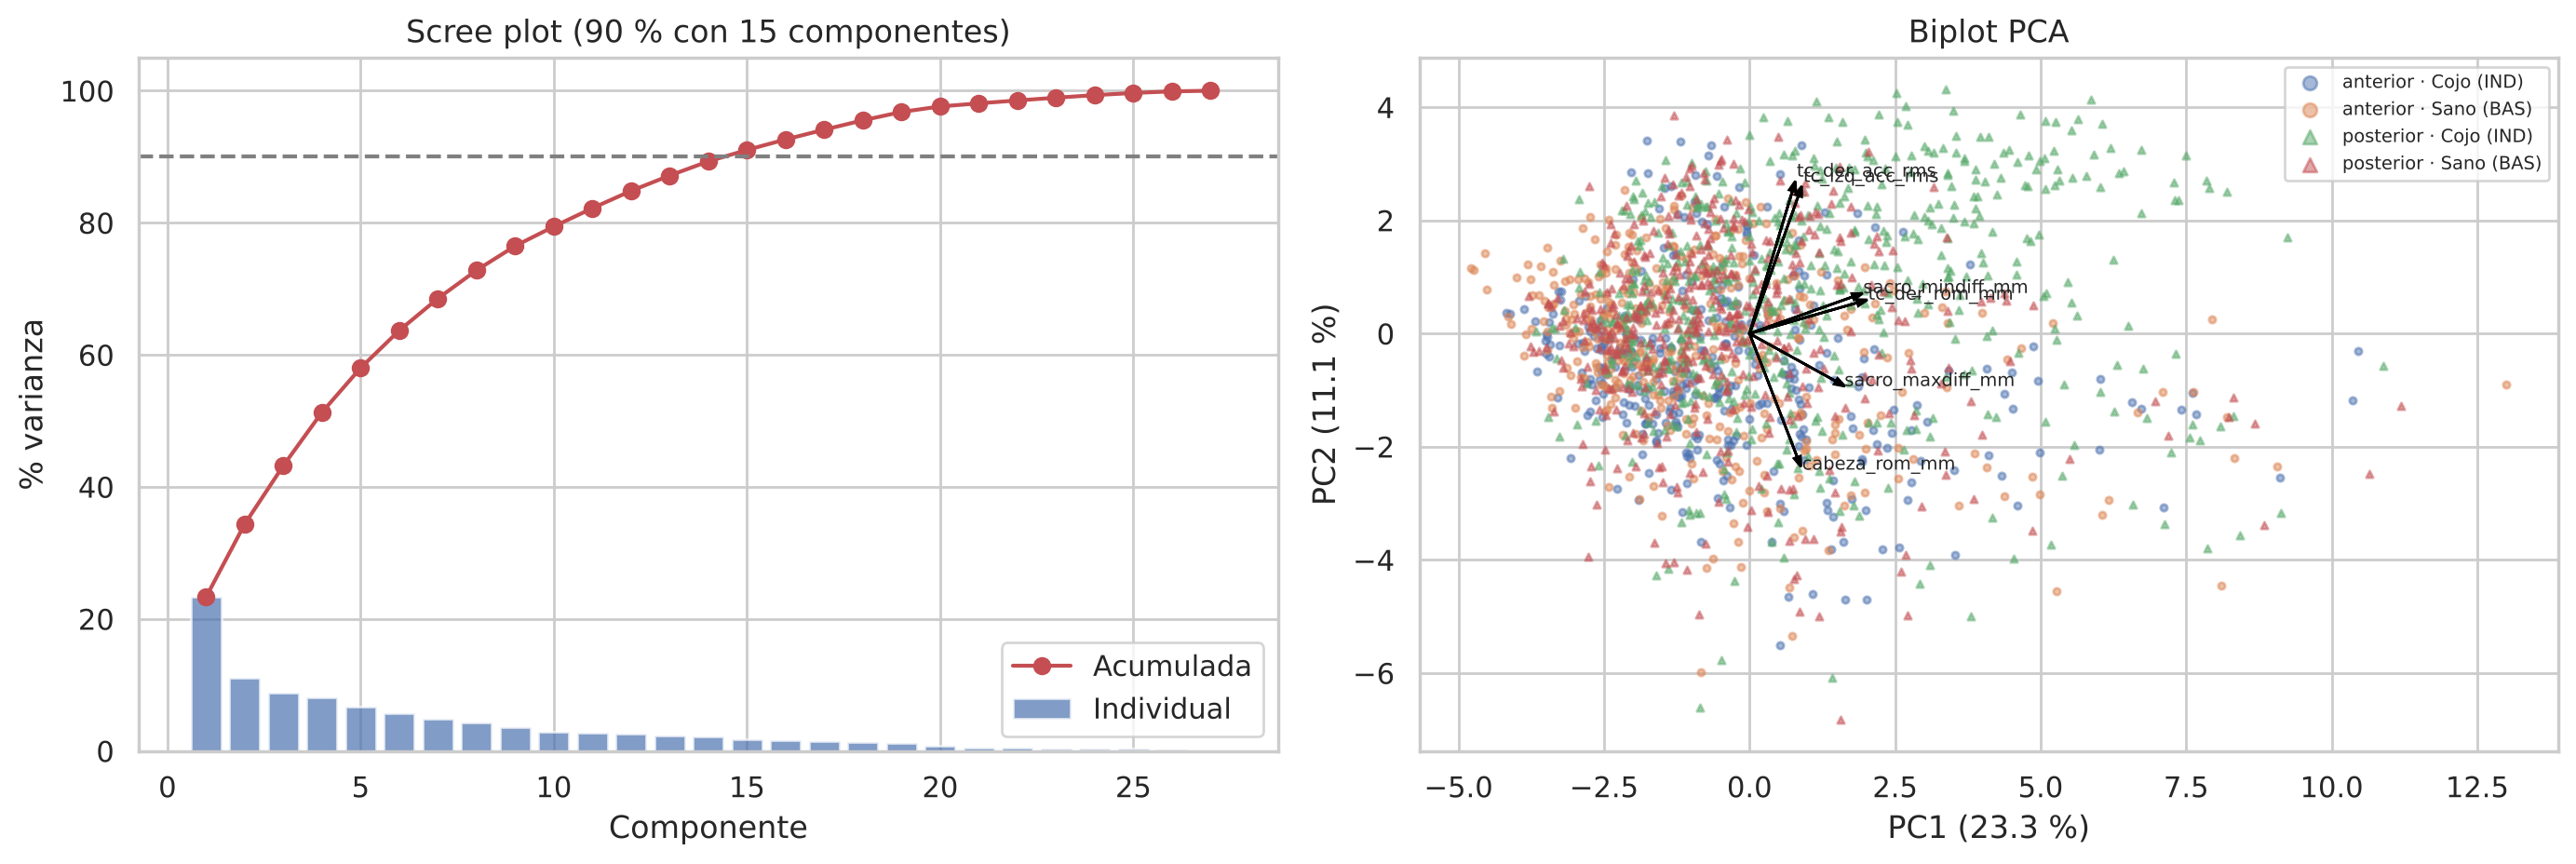
\includegraphics[width=\columnwidth]{imu_pca.png}
\caption{Varianza explicada por PCA y proyección de las zancadas en las dos primeras componentes.}
\label{fig:pca}
\end{figure}

\subsection{Análisis exploratorio y outliers}

El EDA del contenido mostró la evolución temporal, los países, las revistas y el impacto de los artículos. En los sensores, se comparó cada caballo consigo mismo antes y después de la inducción mediante la prueba de Wilcoxon emparejada, que respeta que las zancadas de un mismo animal no son independientes.

Los valores atípicos se interpretaron antes de decidir qué hacer con ellos. En el contenido, los artículos de mayor impacto resultaron ser las herramientas de visión por computador más usadas del área, su frontera tecnológica, así que se conservaron. En los sensores se usó Isolation Forest, esto mostró que las zancadas anómalas se concentran en los caballos cojos, lo que indica que la anomalía es la señal clínica en sí misma, así que solo se eliminaron los registros imposibles y el ruido real como artículos que no tenían nada que ver con el estudio como pruebas genéticas.

\subsection{Minería no supervisada}

Los resúmenes de los artículos se representaron con TF-IDF luego reducidos con SVD y se agruparon con K-Means, eligiendo el número de grupos con cuatro métricas internas y comparando el resultado con clustering jerárquico y DBSCAN (Fig. 3). Este último fue descartado porque dejaba como ruido casi la mitad de los artículos. Además, las palabras clave se analizaron con reglas de asociación como Apriori y FP-Growth~\cite{agrawal1994,han2000}, que llegaron a los mismos conjuntos frecuentes, mostrando coherencia en el proceso. Por otro lado, el catálogo de datasets se agrupó con distancia de Gower y clustering jerárquico, de donde salieron cuatro perfiles.

\begin{figure}[!htb]
\centering
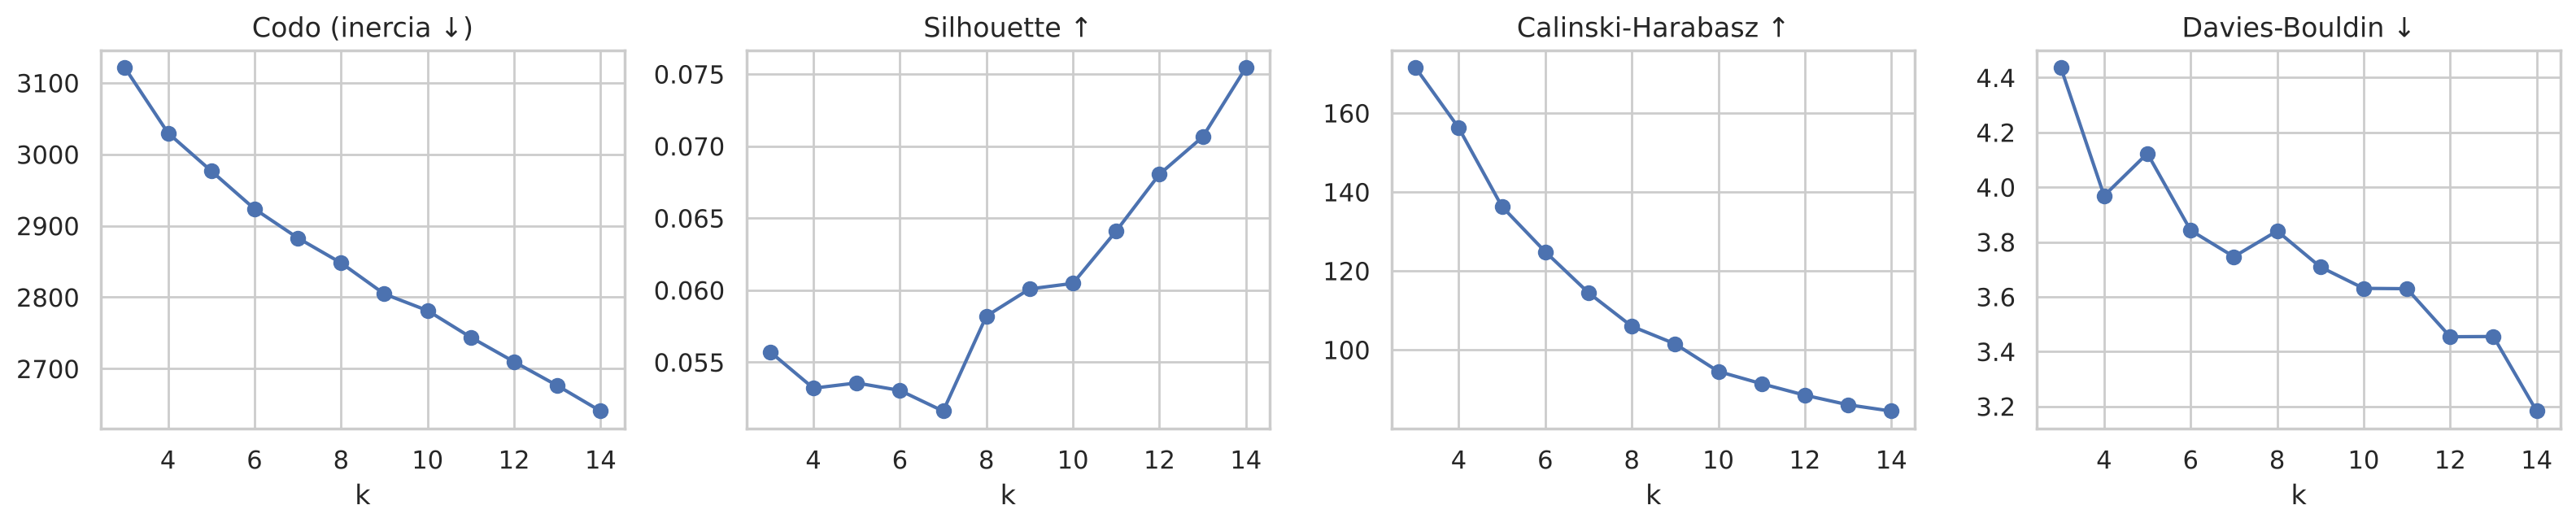
\includegraphics[width=\columnwidth]{art_kmeans_seleccion_k.png}
\caption{Métricas usadas para elegir el número de grupos de K-Means.}
\label{fig:k}
\end{figure}

\section{Modelos de aprendizaje automático}

\subsection{Clasificador de cojera}

El modelo principal clasifica cada zancada como sana o coja, de tal forma que la decisión se \emph{valide con caballos que el modelo no ha evaluado}, las zancadas de un mismo animal presentan alta similitud por lo que mezclarlas entre entrenamiento y prueba haría que el modelo reconociera al caballo y no a la cojera como tal. Por eso se reservaron cinco caballos completos para la prueba final, la selección de modelos se hizo con validación cruzada agrupada por caballo y la robustez fue comprobada dejando cada vez un caballo fuera.

Todos los modelos comparten un pipeline de imputación, escalado y clasificación, ajustado dentro de cada partición para evitar fugas de información. Se compararon regresión logística, KNN y SVM con los modelos de Random Forest, AdaBoost y Gradient Boosting~\cite{breiman2001}, los hiperparámetros se optimizaron con Grid Search para los modelos mencionados, y se usó también Random Search para SVM. El modelo final pudo interpretarse con SHAP~\cite{lundberg2017}.

\subsection{Regresión del impacto científico}

Como complemento, se modeló el impacto de los artículos, medido como citas por año, a partir de sus características: tema, tipo de documento, colaboración, acceso abierto y perfil temático. Se compararon regresión lineal, polinomial, Ridge, Lasso y Elastic Net~\cite{tibshirani1996,zou2005}, con Grid Search sobre la fuerza de regularización, y un Random Forest para referencia con el objetivo de entender qué tipo de trabajo llega a influir más en el área.

\section{Arquitectura en la nube}

\subsection{Selección y justificación}

Se eligió AWS para hacer un despliegue de nube pública. El modelo de servicio usado es principalmente \emph{FaaS} y \emph{PaaS}, usando funciones Lambda y servicios gestionados, esto por la naturaleza intermitente de la carga, que semanalmente repite el ciclo si está activada. Por la misma razón se eligió DynamoDB bajo demanda.

\subsection{Componentes}

La arquitectura de la Fig. 4 tiene cuatro bloques. En la \emph{ingesta}, EventBridge activa cada semana una Lambda que ejecuta el web scraping, con la clave de la API guardada cifrada. El \emph{data lake} en S3 se organiza en zonas de datos \textbf{crudos}, \textbf{procesados} y \textbf{modelos}, con cifrado y versionado, el ciclo a su vez archiva datos antiguos. La \emph{analítica} usa Glue y Athena para consultar los datos con SQL directamente sobre S3. Para interactuar se usa una API HTTP que activa una Lambda empaquetada como imagen Docker con scikit-learn; esta carga el modelo desde S3 y registra cada predicción en DynamoDB, lo que permite seguir la evolución de cada caballo, también se tiene activado un CloudWatch que envía alertas por correo y un presupuesto mensual para evitar sobrecostos.

\begin{figure}[!htb]
\centering
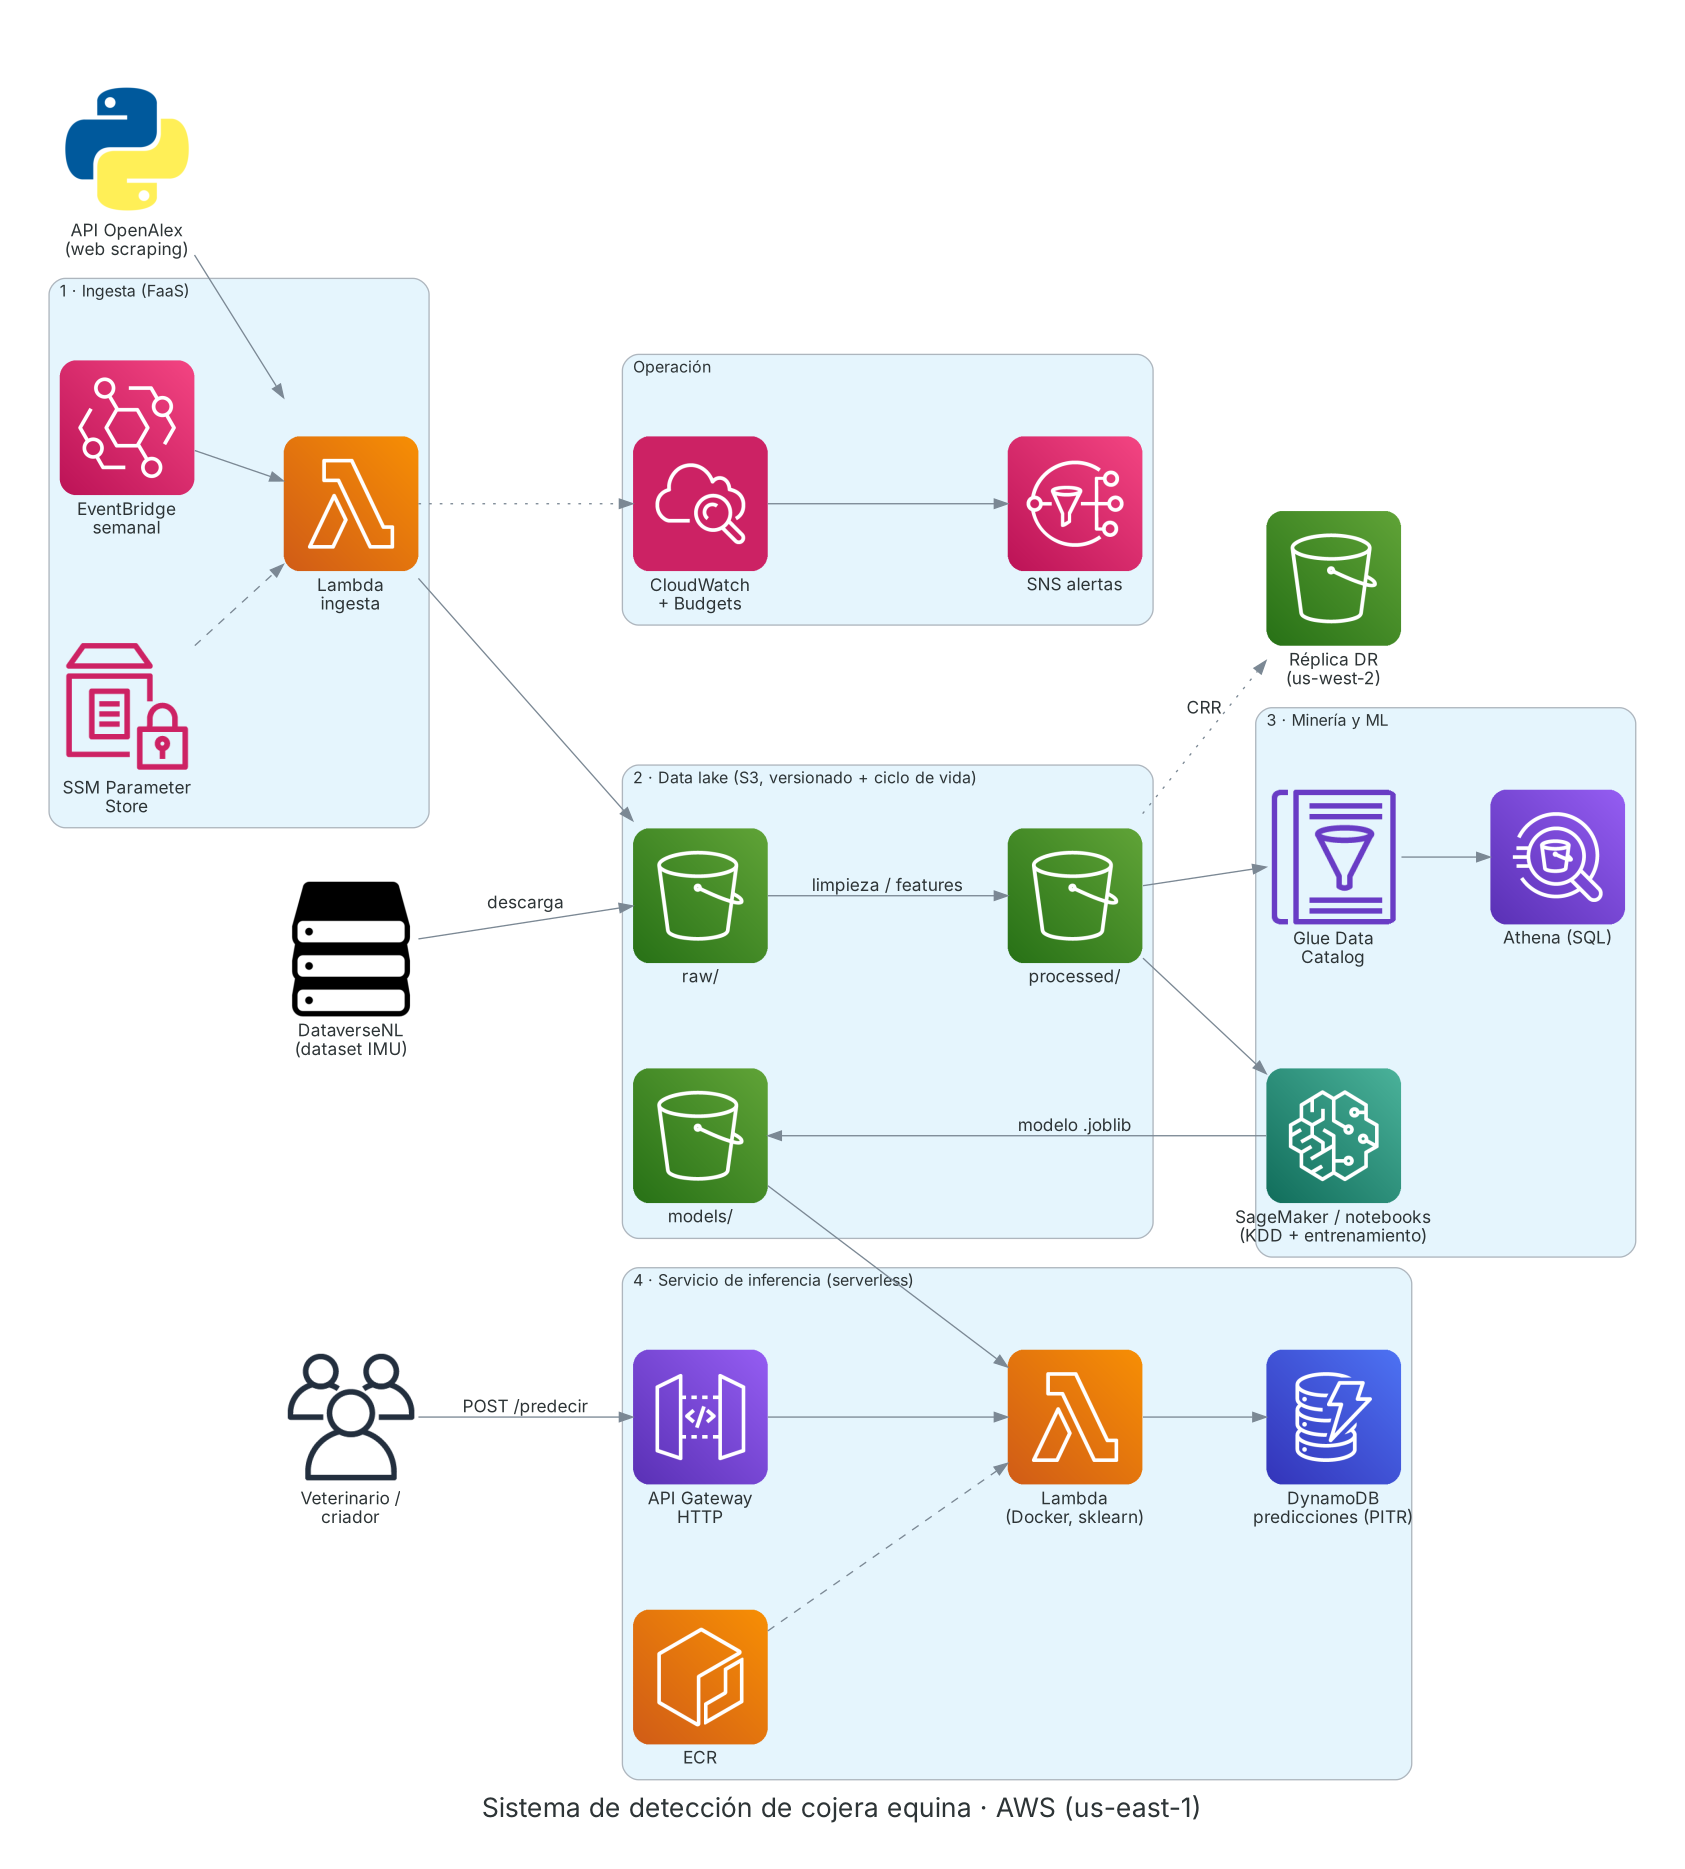
\includegraphics[width=\columnwidth]{arquitectura_aws.png}
\caption{Arquitectura del sistema en AWS.}
\label{fig:aws}
\end{figure}

\subsection{Escalabilidad y recuperación}

Los servicios usados escalan solos según la demanda y funcionan en varias zonas de disponibilidad, por lo que no fue necesario configurar autoescalado ni balanceo de carga. Para recuperar datos, S3 guarda versiones de cada archivo y DynamoDB se puede restaurar a cualquier punto de los últimos 35 días, además, como todo está en Terraform, la infraestructura se puede volver a crear fácilmente.

\subsection{Infraestructura como código y despliegue}

La infraestructura se escribió en Terraform~\cite{terraform} y fue desplegada en una cuenta personal de AWS (Fig. 5). La función de ingesta se ejecuta en la nube y almacena el mismo corpus obtenido de manera local (Fig. 6). En la primera ejecución la función se quedó sin memoria, lo que fue corregido escribiendo los resultados en disco de forma incremental. El incidente muestra el valor de probar el sistema desplegado y no solo el código.

\begin{figure}[!htb]
\centering
\captura{terraform_apply.png}{\columnwidth}
\caption{Despliegue de la infraestructura con Terraform.}
\label{fig:apply}
\end{figure}

\begin{figure}[!htb]
\centering
\captura{s3_openalex.png}{\columnwidth}\\[2mm]
\captura{athena_consulta.png}{\columnwidth}
\caption{Corpus guardado en S3 por la ingesta semanal y consulta SQL en Athena sobre los datos de sensores.}
\label{fig:ingesta}
\end{figure}

\subsection{Integración de extremo a extremo}

La Fig. 7 muestra el funcionamiento completo del sistema, tal que una petición con las medidas de cinco zancadas de un caballo llega a la API, la Lambda aplica el modelo y responde con la probabilidad de cojera, y la predicción queda registrada en DynamoDB. 

\begin{figure}[!htb]
\centering
\captura{api_respuesta.png}{\columnwidth}\\[2mm]
\captura{dynamodb_items.png}{\columnwidth}
\caption{Respuesta de la API de inferencia y predicción registrada en DynamoDB.}
\label{fig:api}
\end{figure}

\section{Resultados}

\subsection{Estado del arte}

La producción científica crece constantemente y, en los últimos años, la visión por computador tomó la dominancia como enfoque investigativo frente a los estudios clínicos tradicionales (Fig. 8). Al aplicar clustering se identificaron ocho líneas de investigación que separan un grupo clínico antiguo de uno más tecnológico, reciente y con mayor impacto, formado por estimación de pose, visión, sensores y detección en bovinos (Fig. 9). Las reglas de asociación mostraron que los métodos de pose animal  son heredados de los de pose humana y que la detección automática de cojera ha sido desarrollada sobre todo en vacas lecheras. El vacío evidenciado tras la investigación es que, de los trabajos que combinan caballo, cojera y visión por computador, apenas uno tiene autores en Colombia.

\begin{figure}[!htb]
\centering
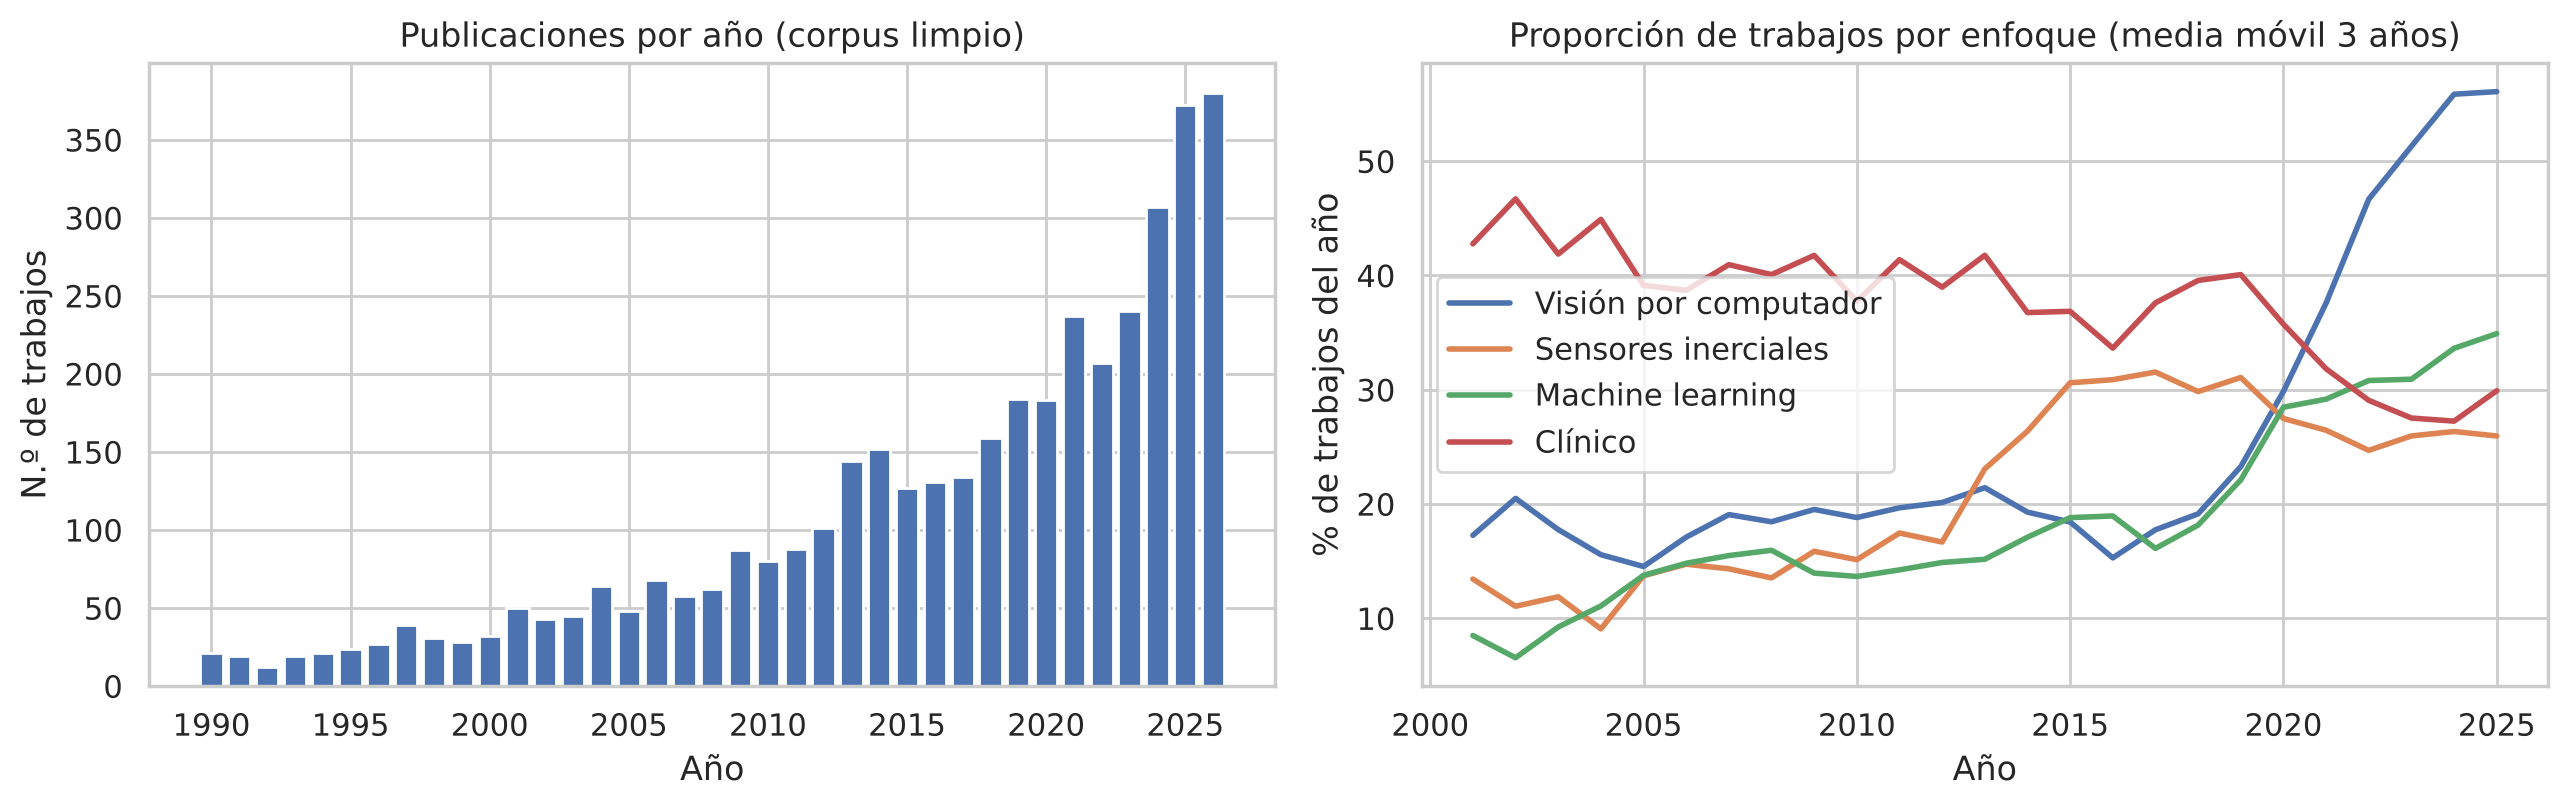
\includegraphics[width=\columnwidth]{art_tendencia_anual.png}
\caption{Publicaciones por año y proporción de trabajos según su enfoque. El año 2026 está incompleto.}
\label{fig:tendencia}
\end{figure}

\begin{figure}[!htb]
\centering
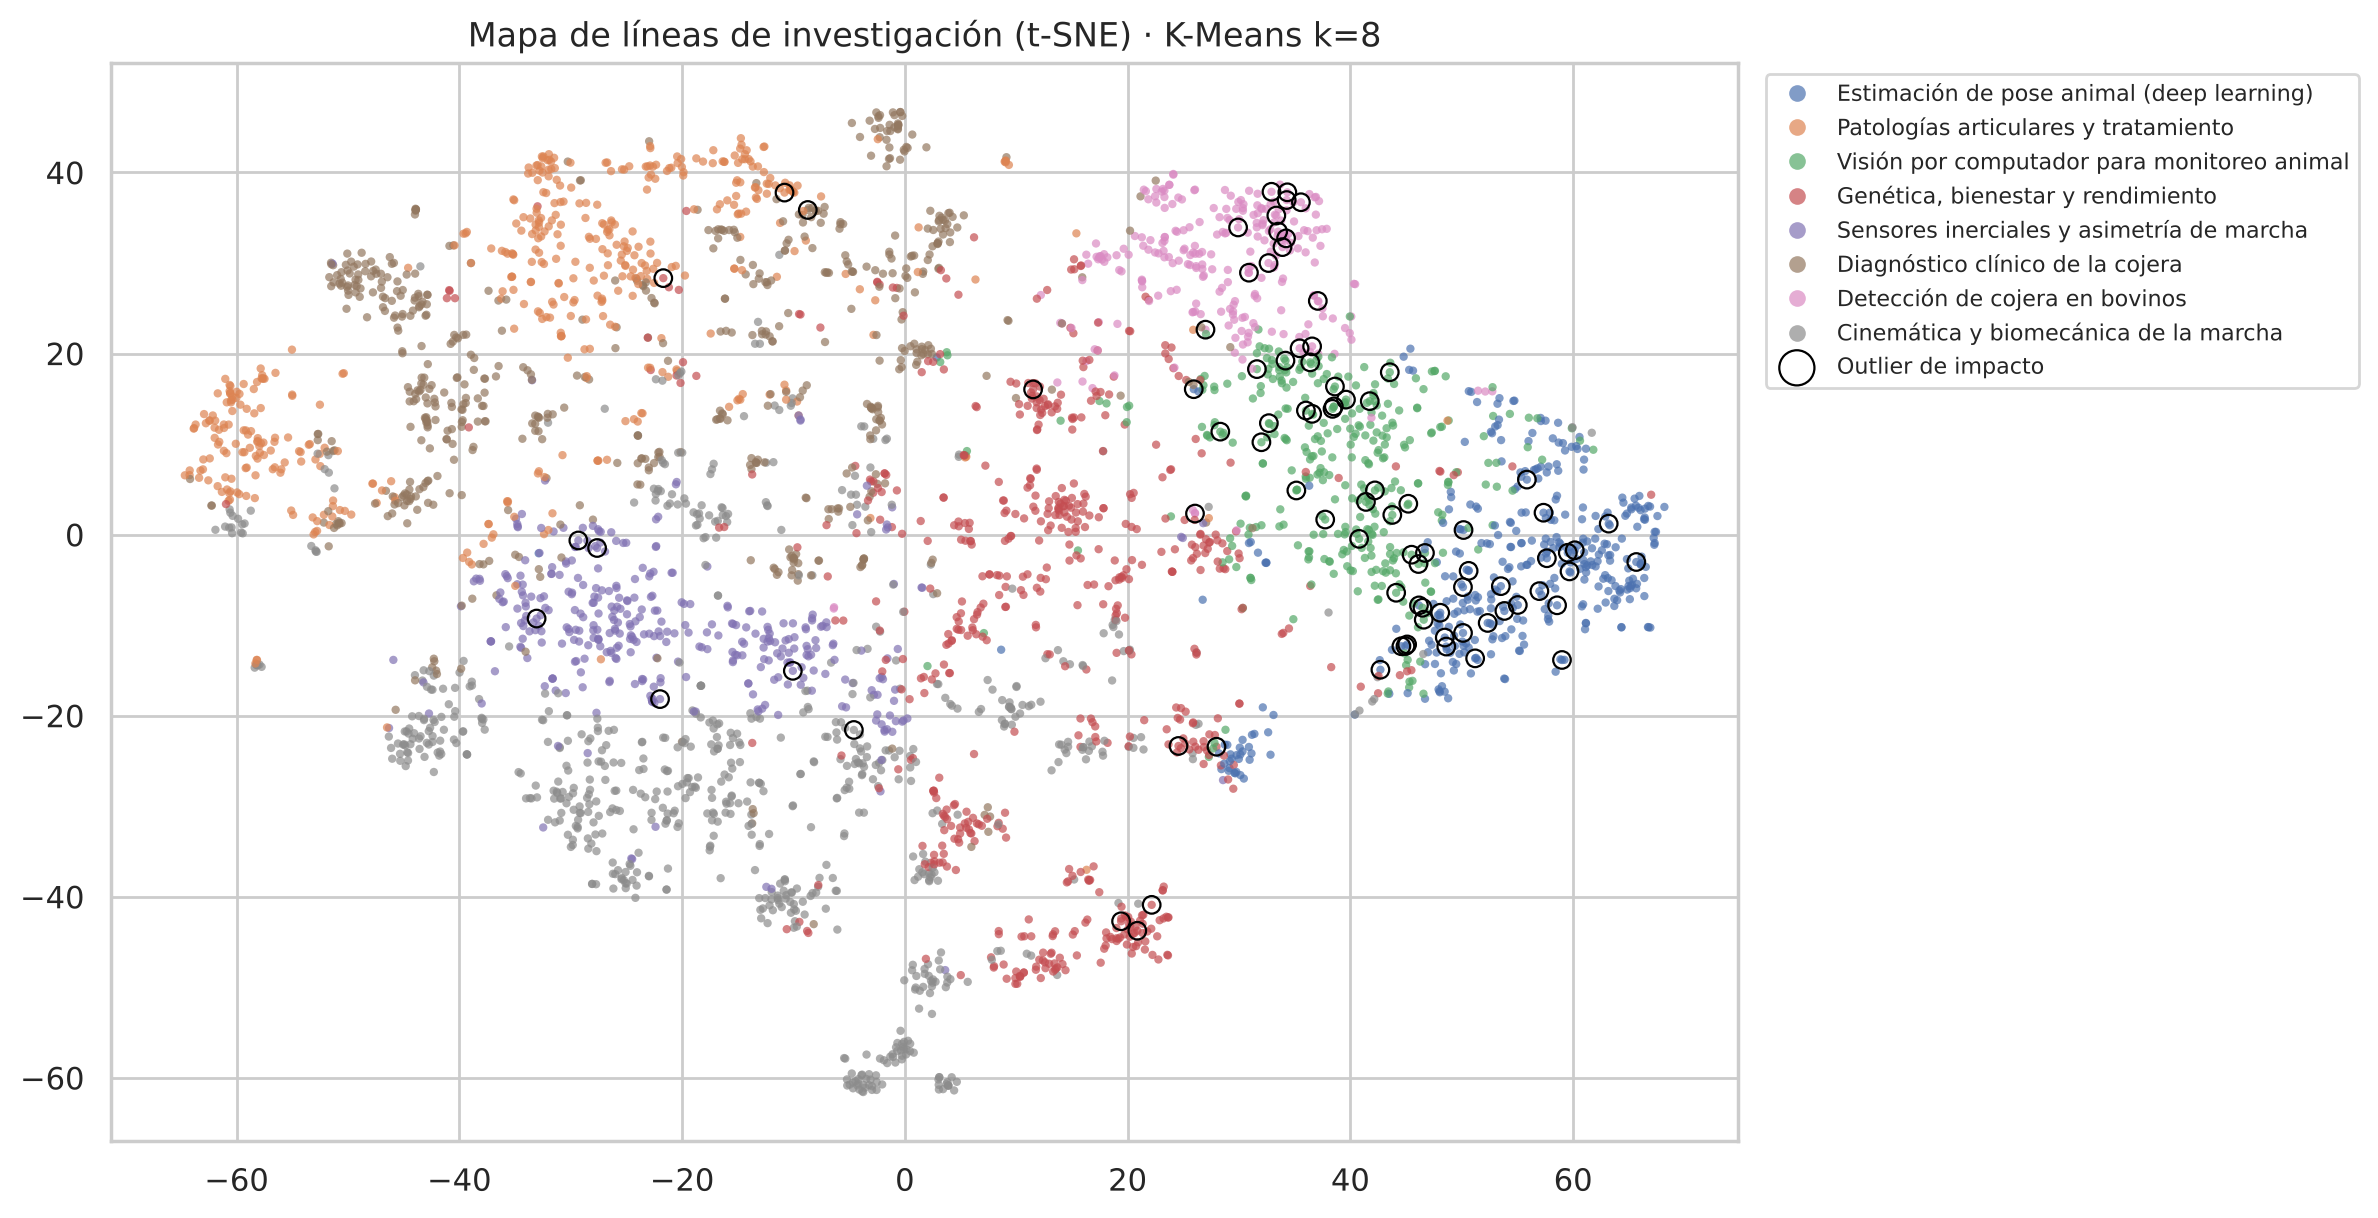
\includegraphics[width=\columnwidth]{art_tsne_clusters.png}
\caption{Mapa de las líneas de investigación encontradas por clustering. Los círculos negros marcan los trabajos de impacto atípico.}
\label{fig:tsne}
\end{figure}

\subsection{Datasets disponibles}

El catálogo se organizó en cuatro perfiles: captura de movimiento de caballos, sensores con etiqueta de cojera, imágenes de pose y videos con puntos anatómicos. Ningún dataset público combina video de caballos con etiqueta de cojera (Fig. 10). Esto define la estrategia para una posterior fase de visión: aprender a ubicar los puntos anatómicos con Horse-10 o AP-10K, comprobar las trayectorias contra la captura de movimiento de PFERD y aplicar el clasificador de este trabajo.

\begin{figure}[!htb]
\centering
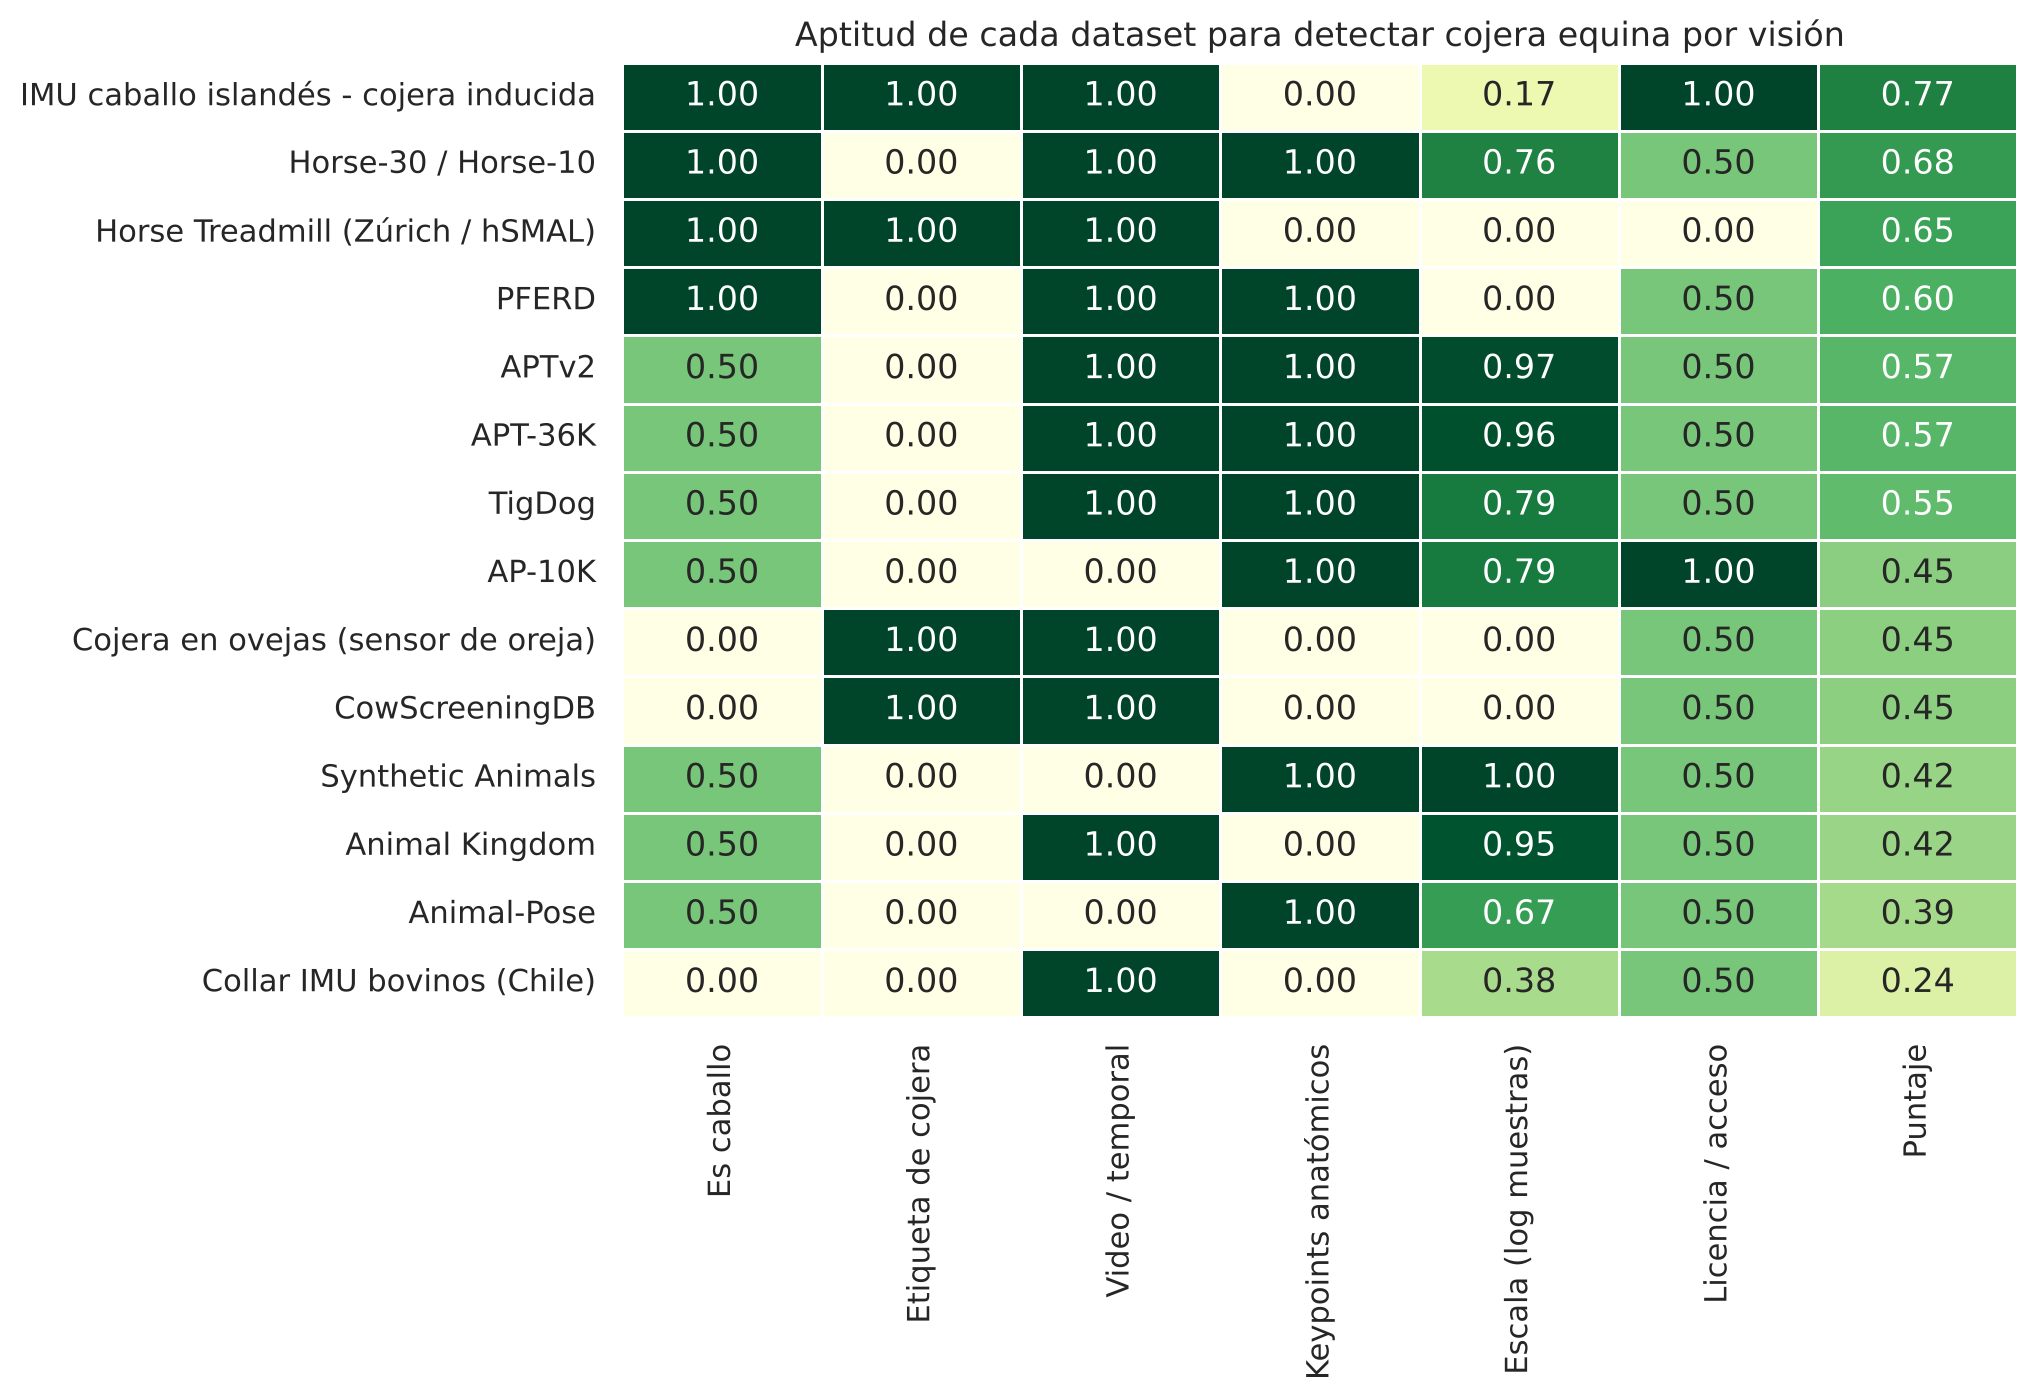
\includegraphics[width=0.9\columnwidth]{cat_matriz_aptitud.png}
\caption{Aptitud de cada dataset público para el objetivo del proyecto.}
\label{fig:aptitud}
\end{figure}

\subsection{Señales de la marcha}

Al comparar cada caballo consigo mismo, la cojera anterior casi duplicó la asimetría de la cabeza, mientras que la cojera posterior aumentó la asimetría del sacro y la diferencia entre caderas, con diferencias estadísticamente significativas (Figs. 11 y 12). Este patrón lo describe la clínica de manera que el caballo levanta la cabeza al apoyar una pata delantera dolorida, y la cadera cuando el dolor está atrás. La respuesta varía entre individuos, y algunos caballos son asimétricos incluso sanos. El clustering de caballos lo confirmó: separó en buena medida a los sanos de los cojos, salvo justamente a esos individuos. Por eso un umbral fijo no cumple con la tarea.

\begin{figure}[H]
\centering
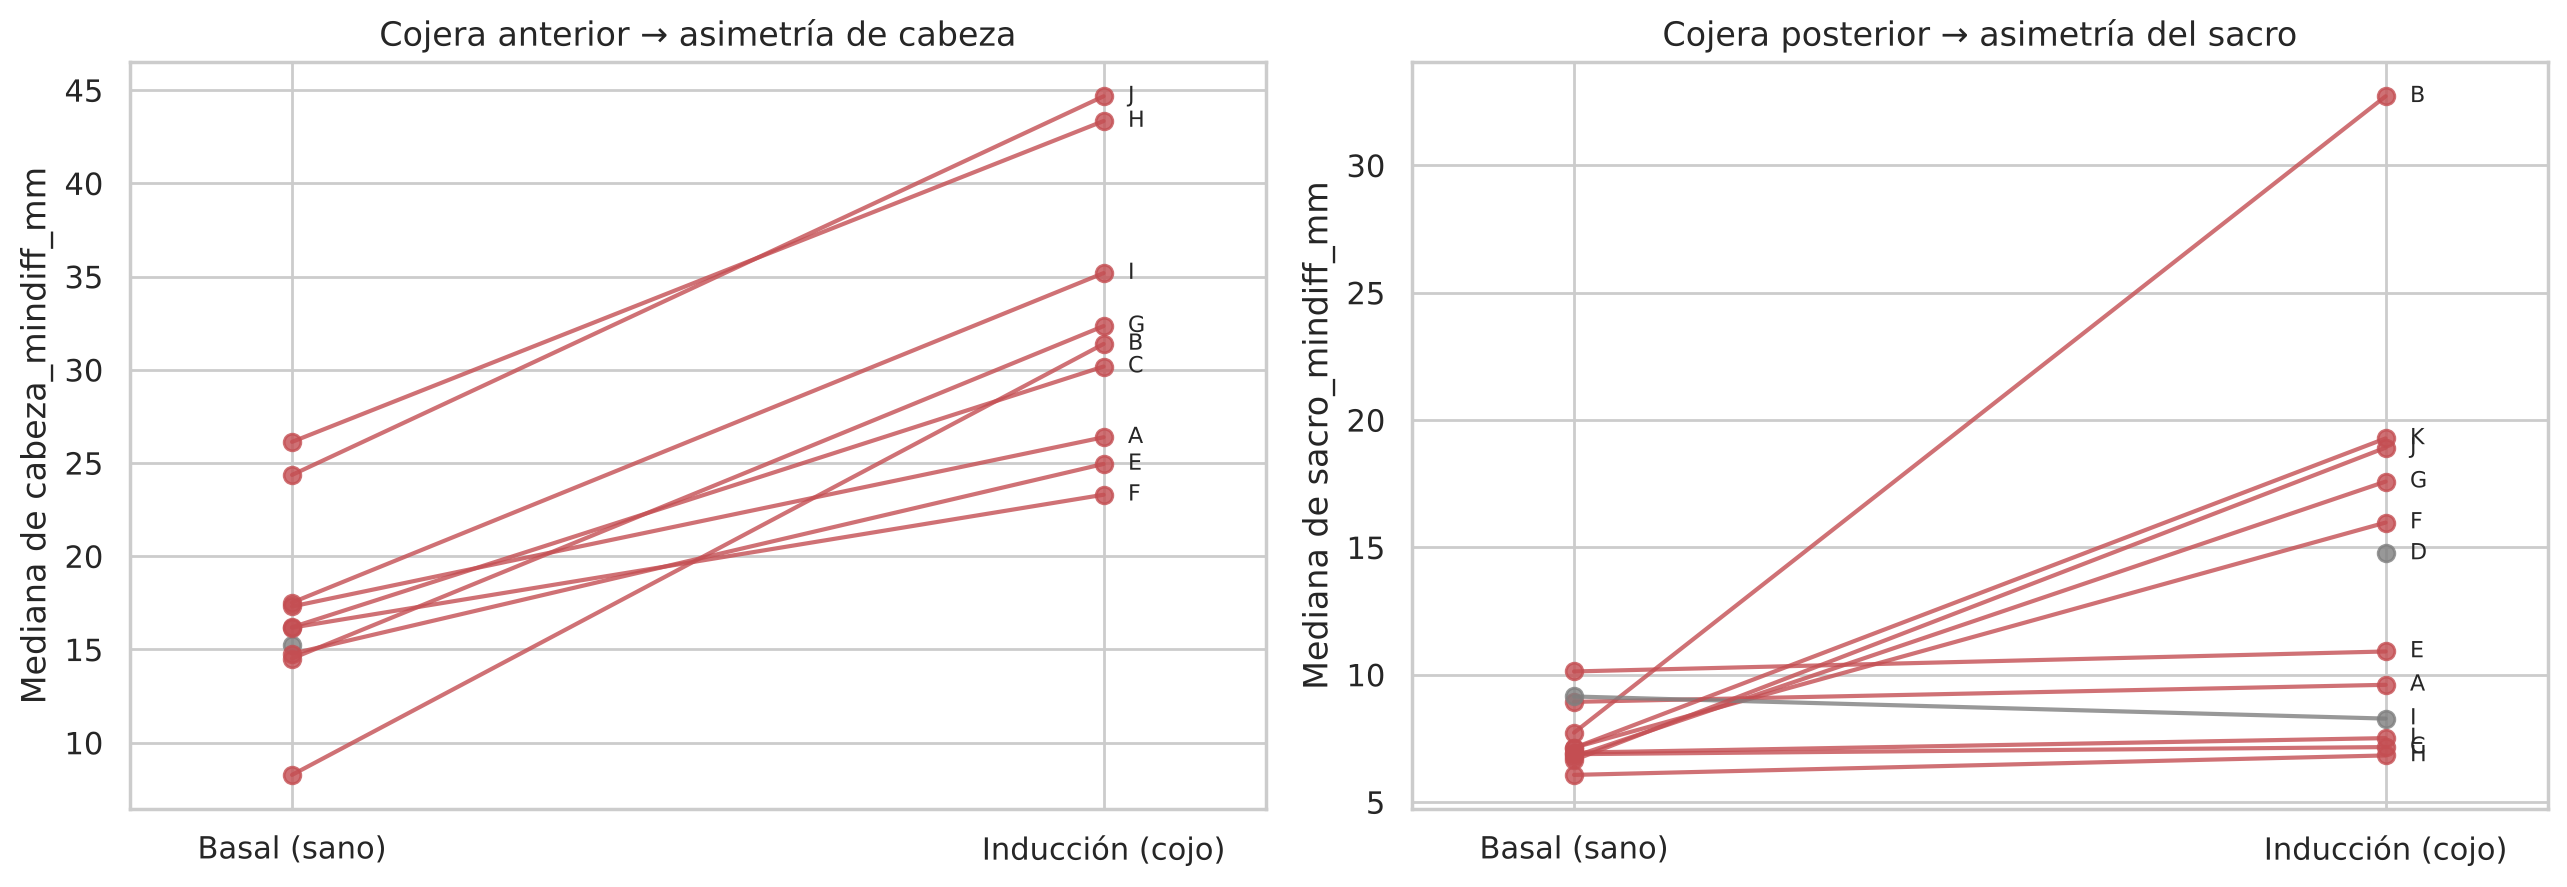
\includegraphics[width=\columnwidth]{imu_pareado_caballos.png}
\caption{Cambio de la asimetría de cada caballo entre la condición sana y la cojera inducida.}
\label{fig:pareado}
\end{figure}

\begin{figure}[H]
\centering
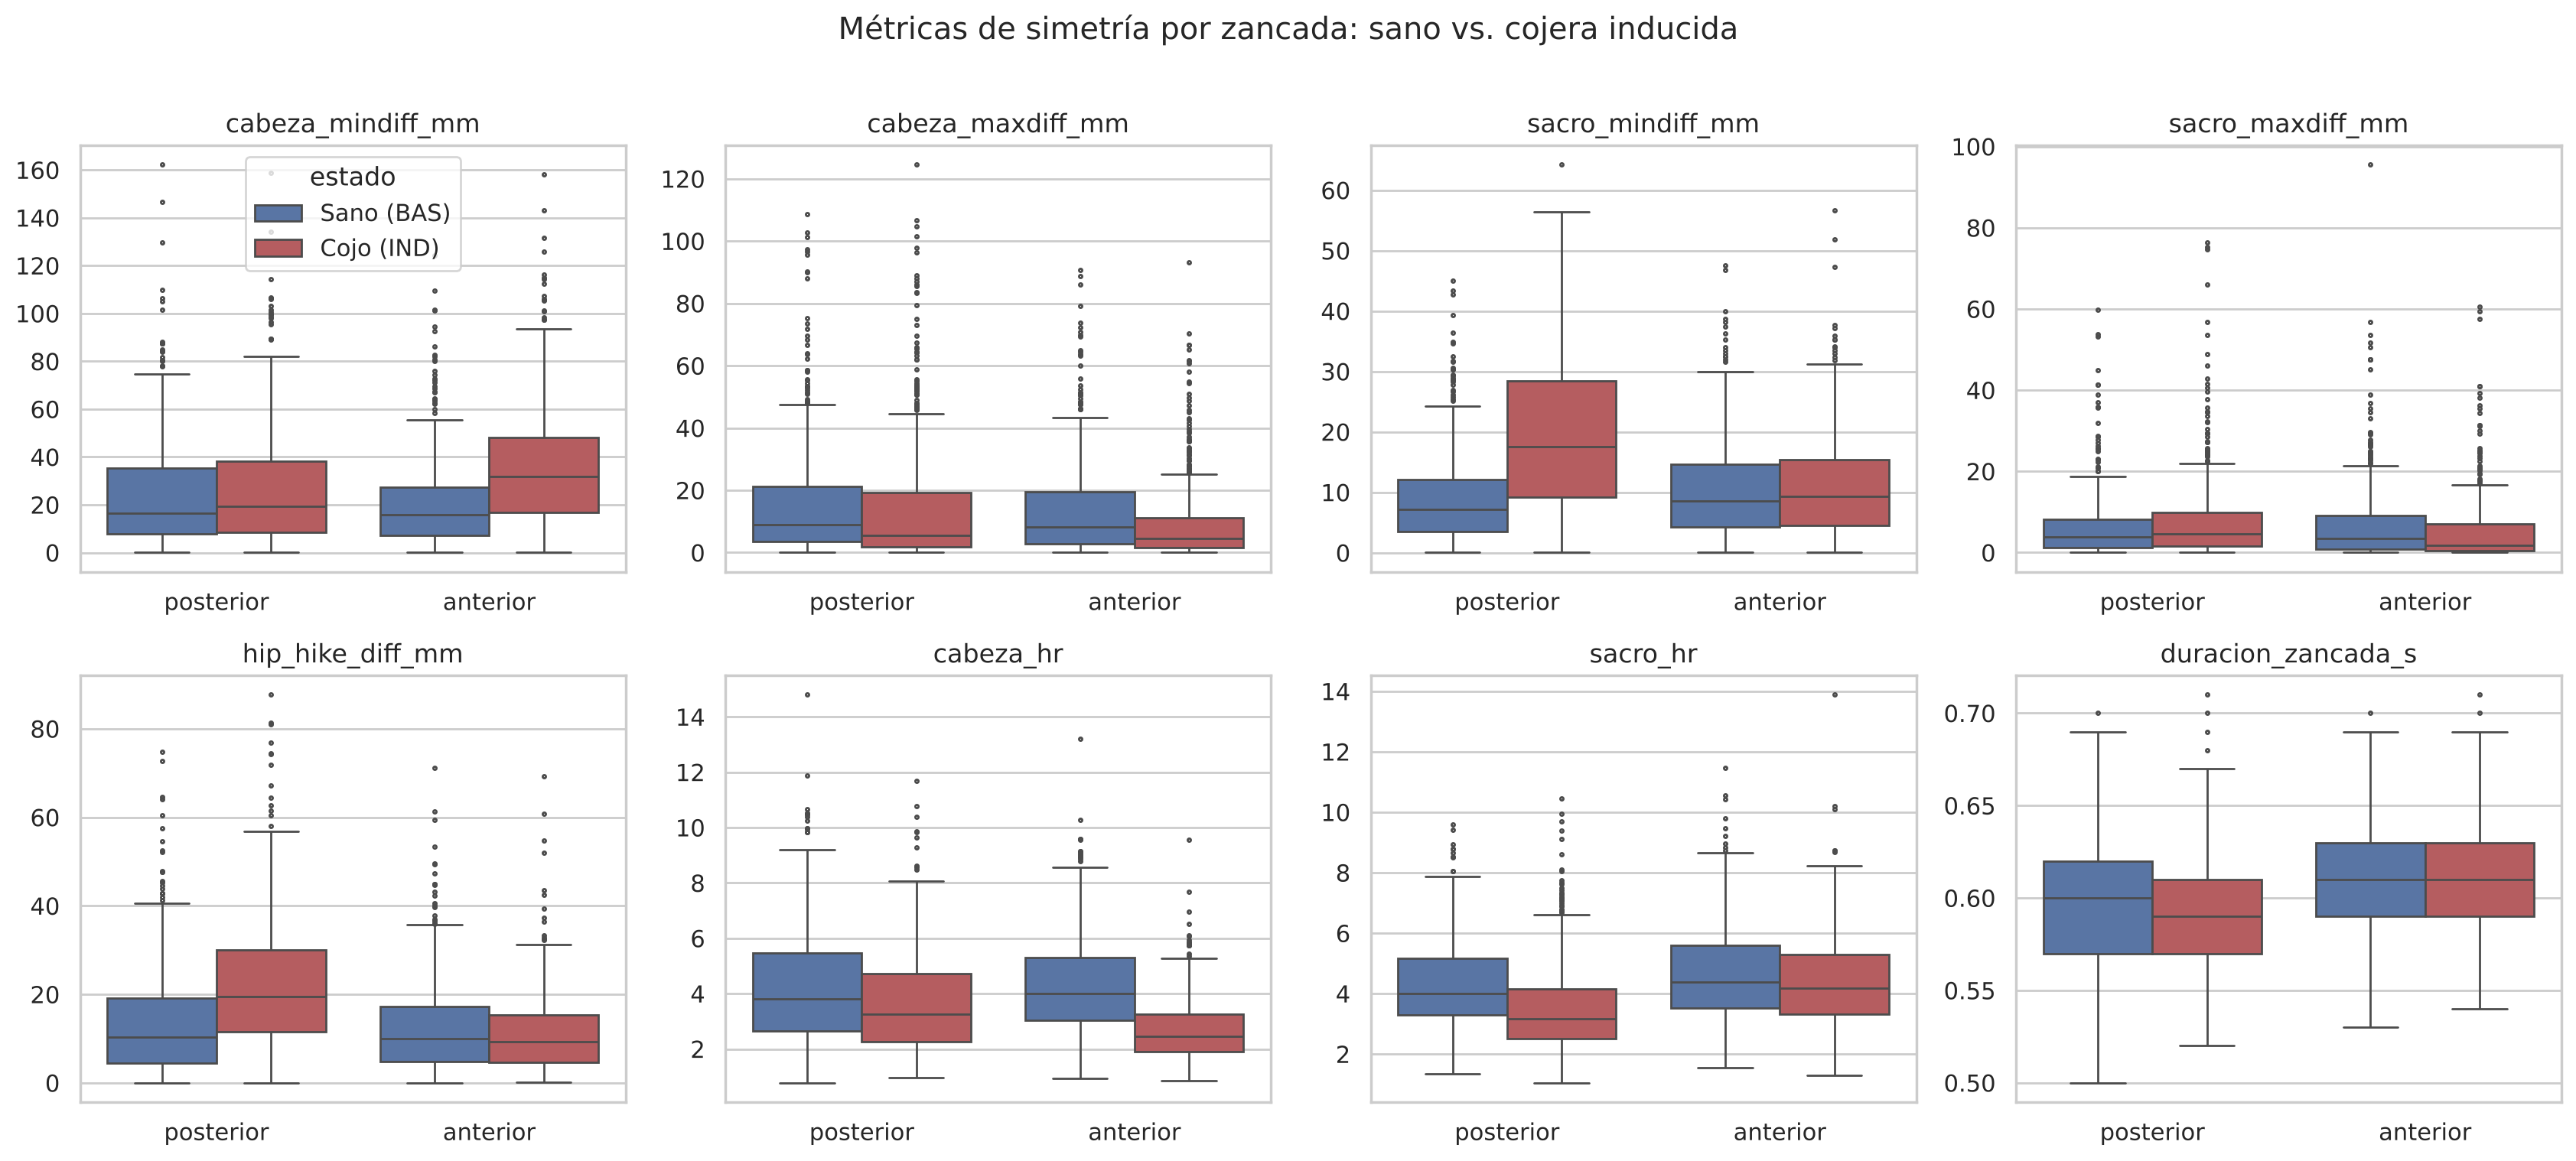
\includegraphics[width=\columnwidth]{imu_boxplots.png}
\caption{Distribución de las métricas de simetría por zancada en caballos sanos y con cojera inducida, por tipo de cojera.}
\label{fig:box}
\end{figure}

\subsection{Clasificador de cojera}

La Tabla I resume los resultados. En validación cruzada los modelos quedaron cerca entre sí, y Random Forest fue el mejor tras la optimización, por lo que se eligió como modelo final por su desempeño, su interpretabilidad exacta con SHAP además que tiene un bajo costo de cómputo. Con los cinco caballos de prueba alcanzó un ROC-AUC de 0,71, el mismo valor obtenido dejando cada vez un caballo fuera, y al promediar las zancadas de cada prueba de trote acertó siete de nueve (Fig. 13). Gradient Boosting rindió un poco mejor en la prueba, pero no se eligió, porque el modelo se selecciona con la validación y no mirando el conjunto de prueba. SHAP muestra que el modelo se apoya en la asimetría del sacro, la regularidad del movimiento de la cabeza y la diferencia entre caderas, los mismos marcadores que usa un veterinario (Fig. 14). El desempeño es moderado, como cabe esperar con cojeras leves evaluadas en caballos nuevos, y es una estimación honesta de cómo funcionaría el sistema en la práctica.

\begin{table}[H]
\centering
\caption{Clasificación con validación agrupada por caballo (ROC-AUC)}
\label{tab:ml}
\begin{tabular}{lcc}
\toprule
Modelo & Validación cruzada & Prueba \\
\midrule
Regresión logística & 0,67 & 0,68 \\
SVM optimizada & 0,68 & 0,69 \\
Gradient Boosting optimizado & 0,63 & 0,72 \\
\textbf{Random Forest optimizado} & \textbf{0,67} & \textbf{0,71} \\
\bottomrule
\end{tabular}
\end{table}

\begin{figure}[!htb]
\centering
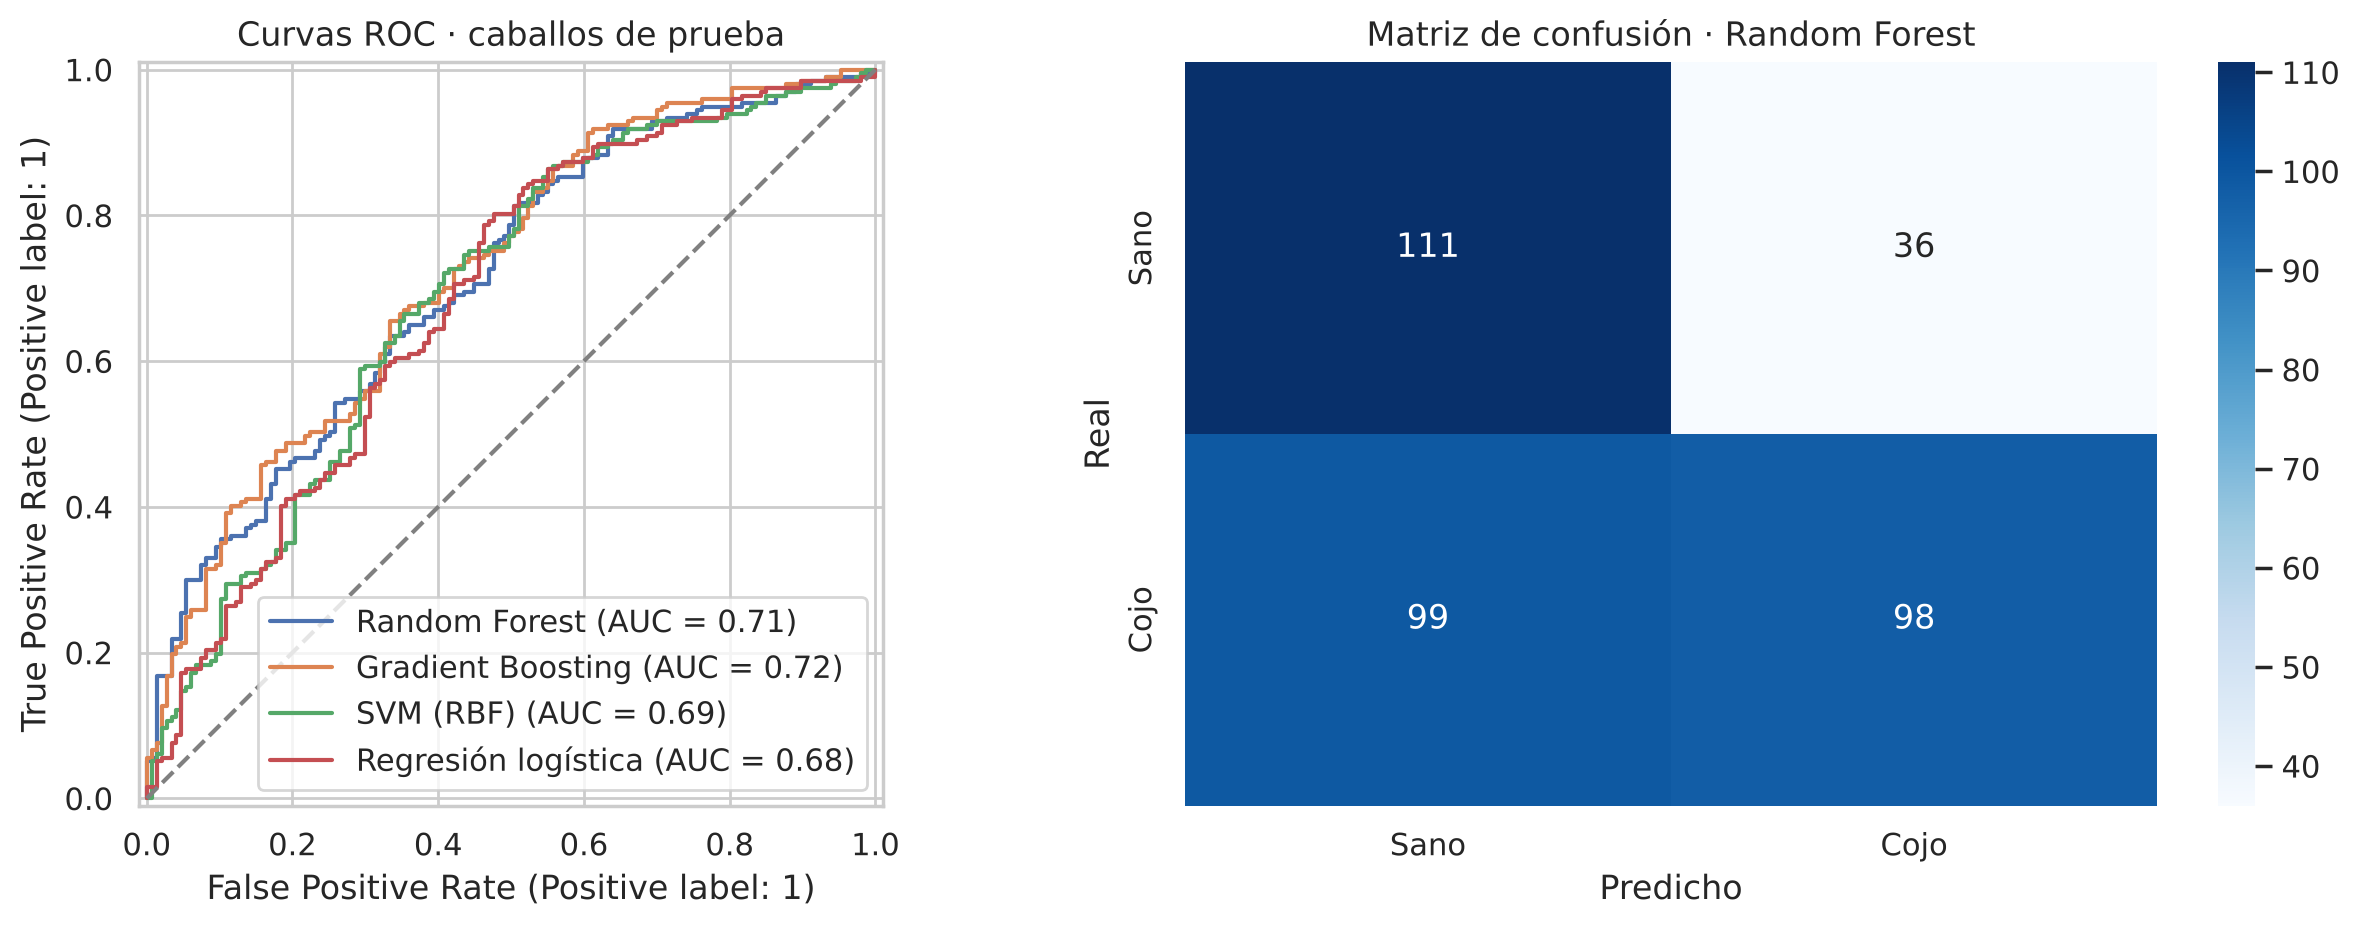
\includegraphics[width=\columnwidth]{ml_roc_confusion.png}
\caption{Curvas ROC con los caballos de prueba y matriz de confusión del modelo final.}
\label{fig:roc}
\end{figure}

\begin{figure}[!htb]
\centering
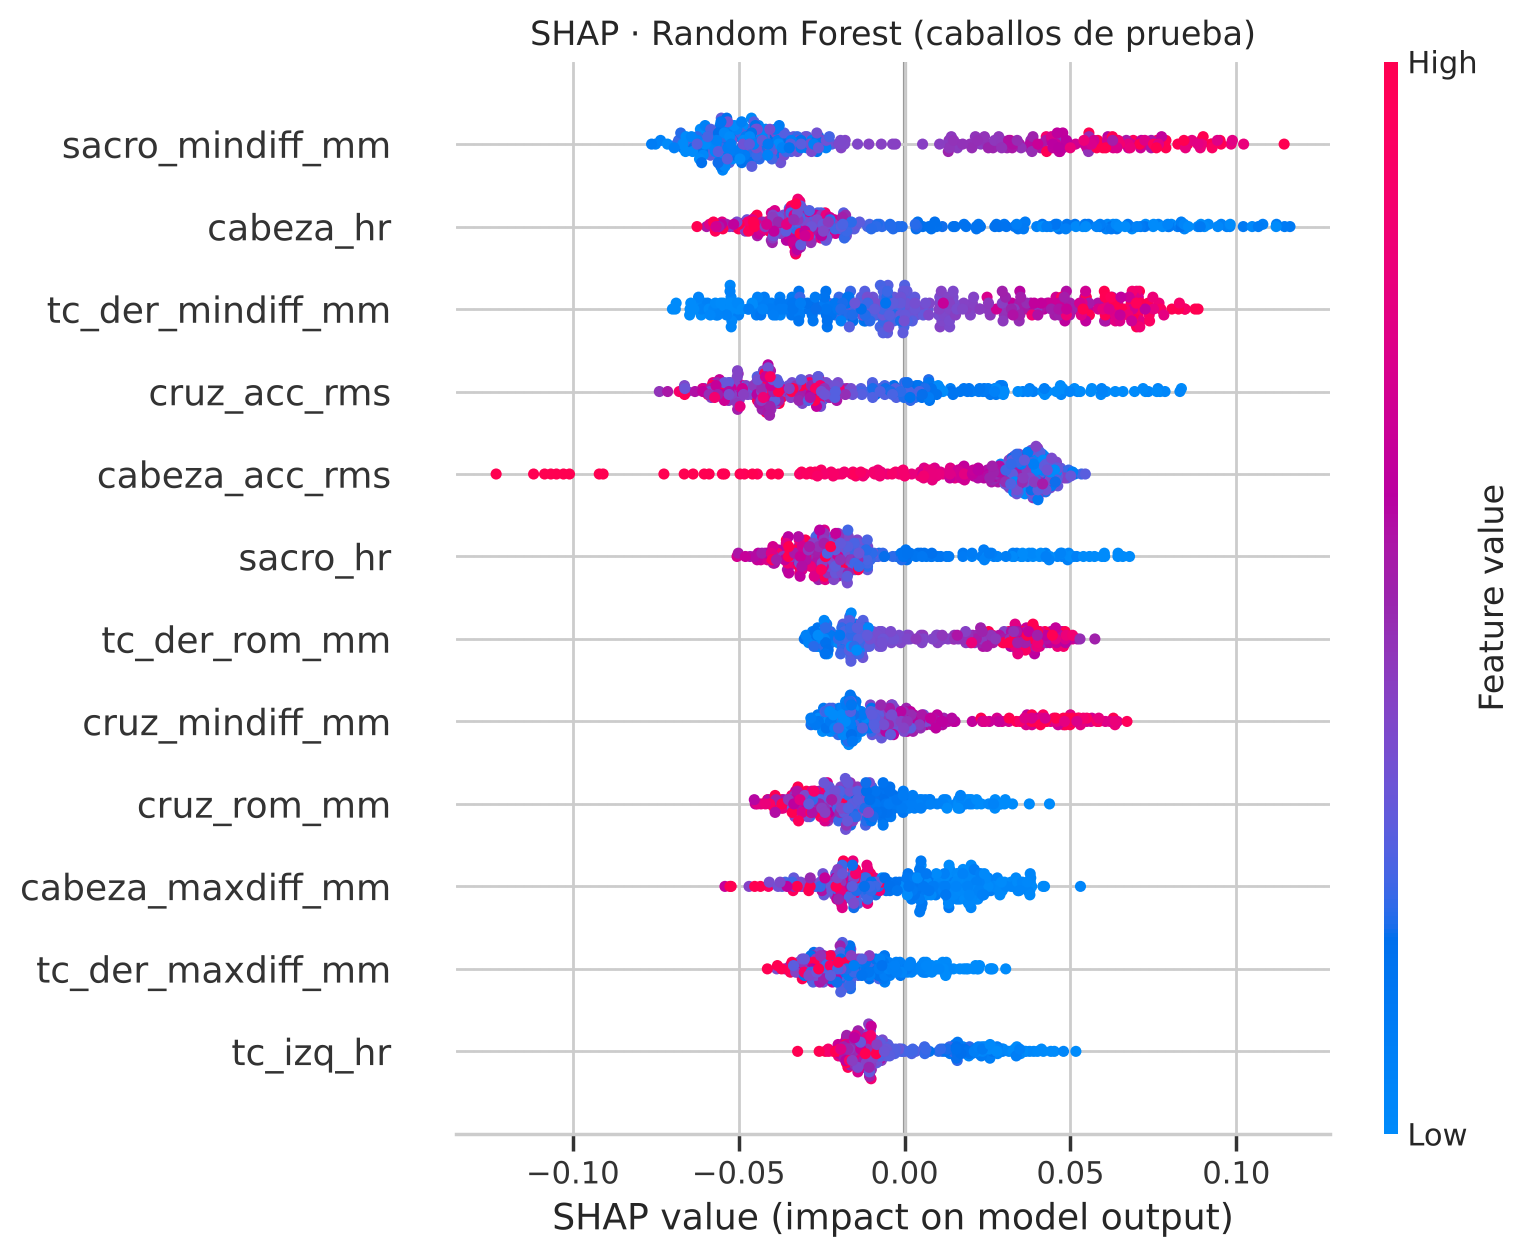
\includegraphics[width=0.85\columnwidth]{ml_shap_summary.png}
\caption{Variables que más influyen en el modelo según SHAP.}
\label{fig:shap}
\end{figure}

\subsection{Impacto científico}

Los modelos lineales explicaron cerca del 40 \% de la variación del impacto, la regresión polinomial regularizada alrededor del 50 \% y el Random Forest algo más, por su capacidad de capturar interacciones (Fig. 15). Ridge, Lasso y Elastic Net rindieron igual que la regresión lineal, porque con tres mil artículos y pocas variables no había sobreajuste que corregir. Su utilidad principal fue seleccionar variables. Lasso mostró que los perfiles de estimación de pose, visión y detección en bovinos, junto con la colaboración entre países, se asocian con más citas por año, y que los perfiles clínicos clásicos se asocian con menos (Fig. 16). Esto refuerza la decisión de orientar el proyecto hacia la visión por computador.

\begin{figure}[!htb]
\centering
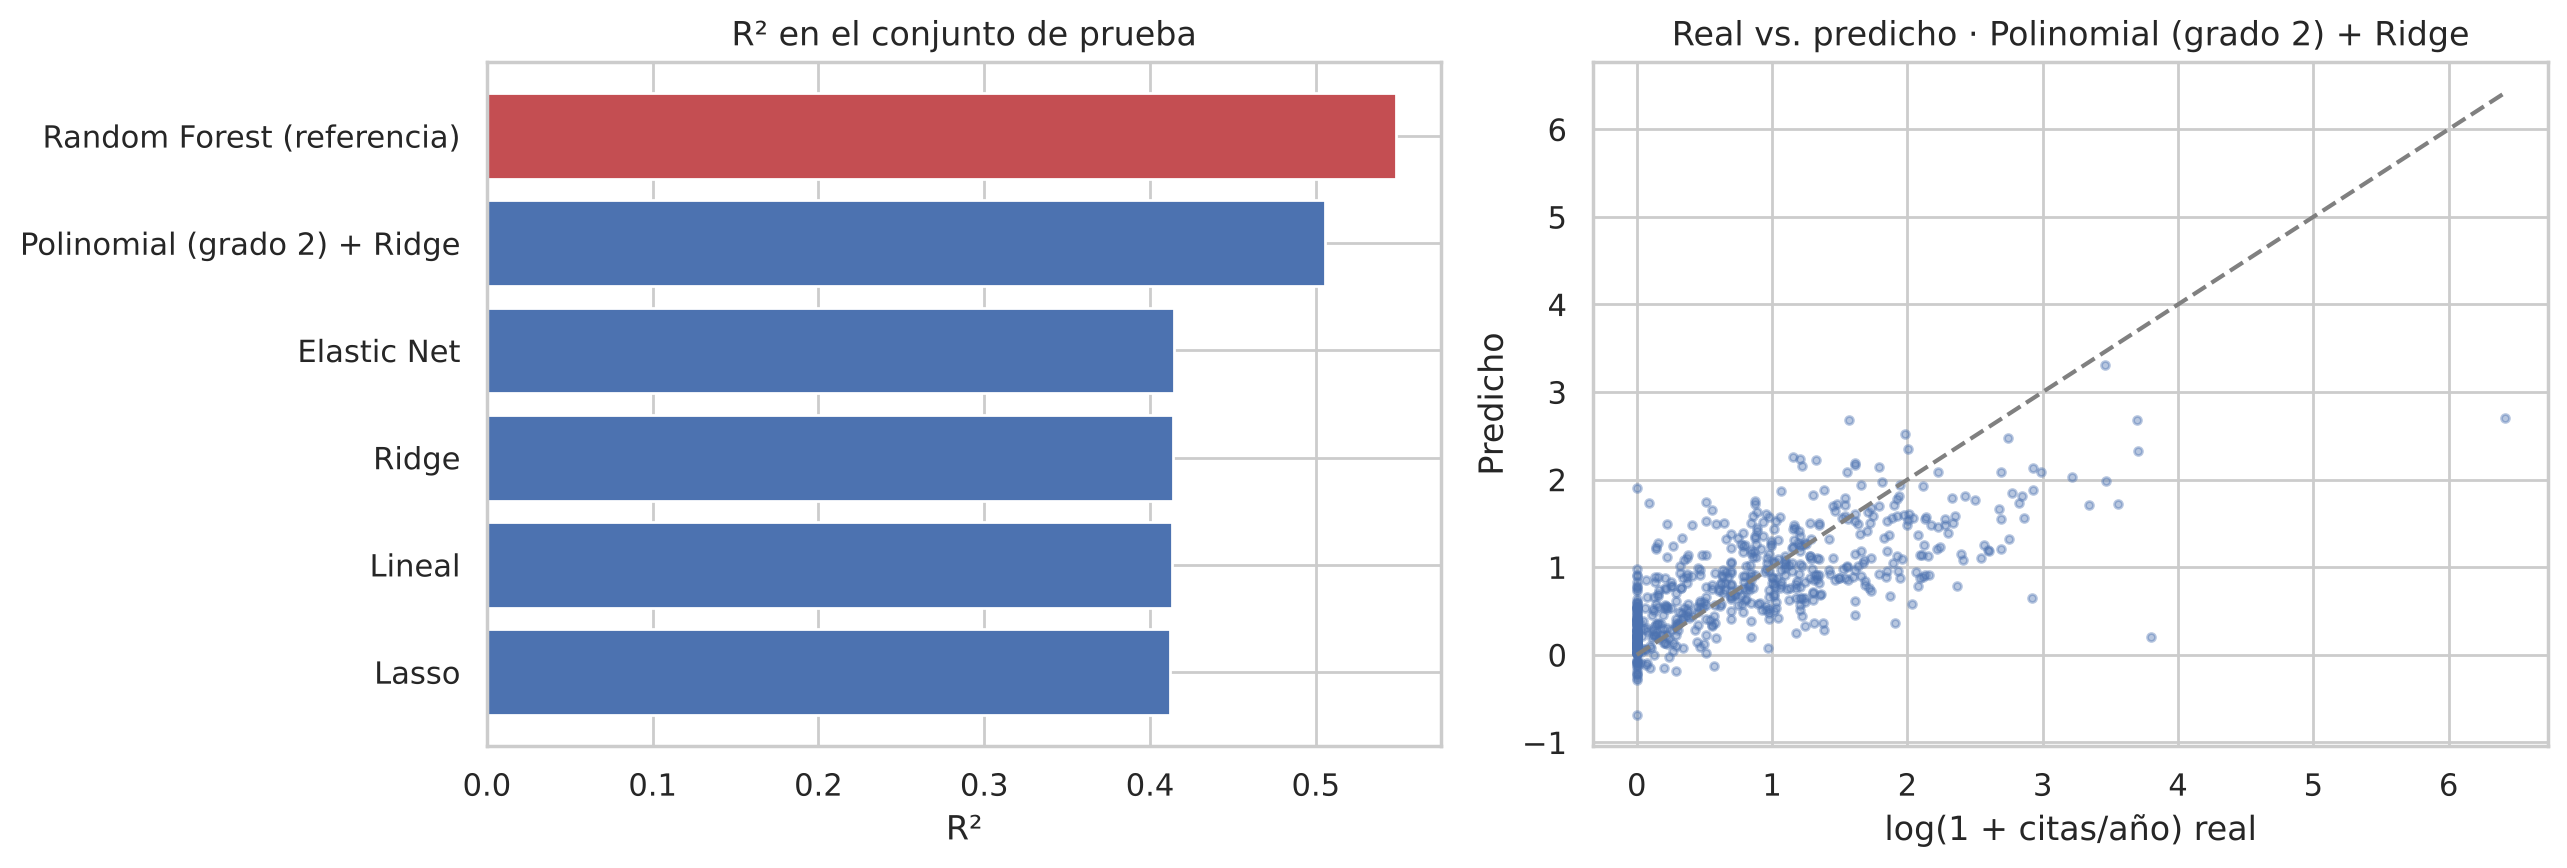
\includegraphics[width=\columnwidth]{reg_comparacion.png}
\caption{Comparación de los modelos de regresión y valores reales frente a predichos.}
\label{fig:reg}
\end{figure}

\begin{figure}[!htb]
\centering
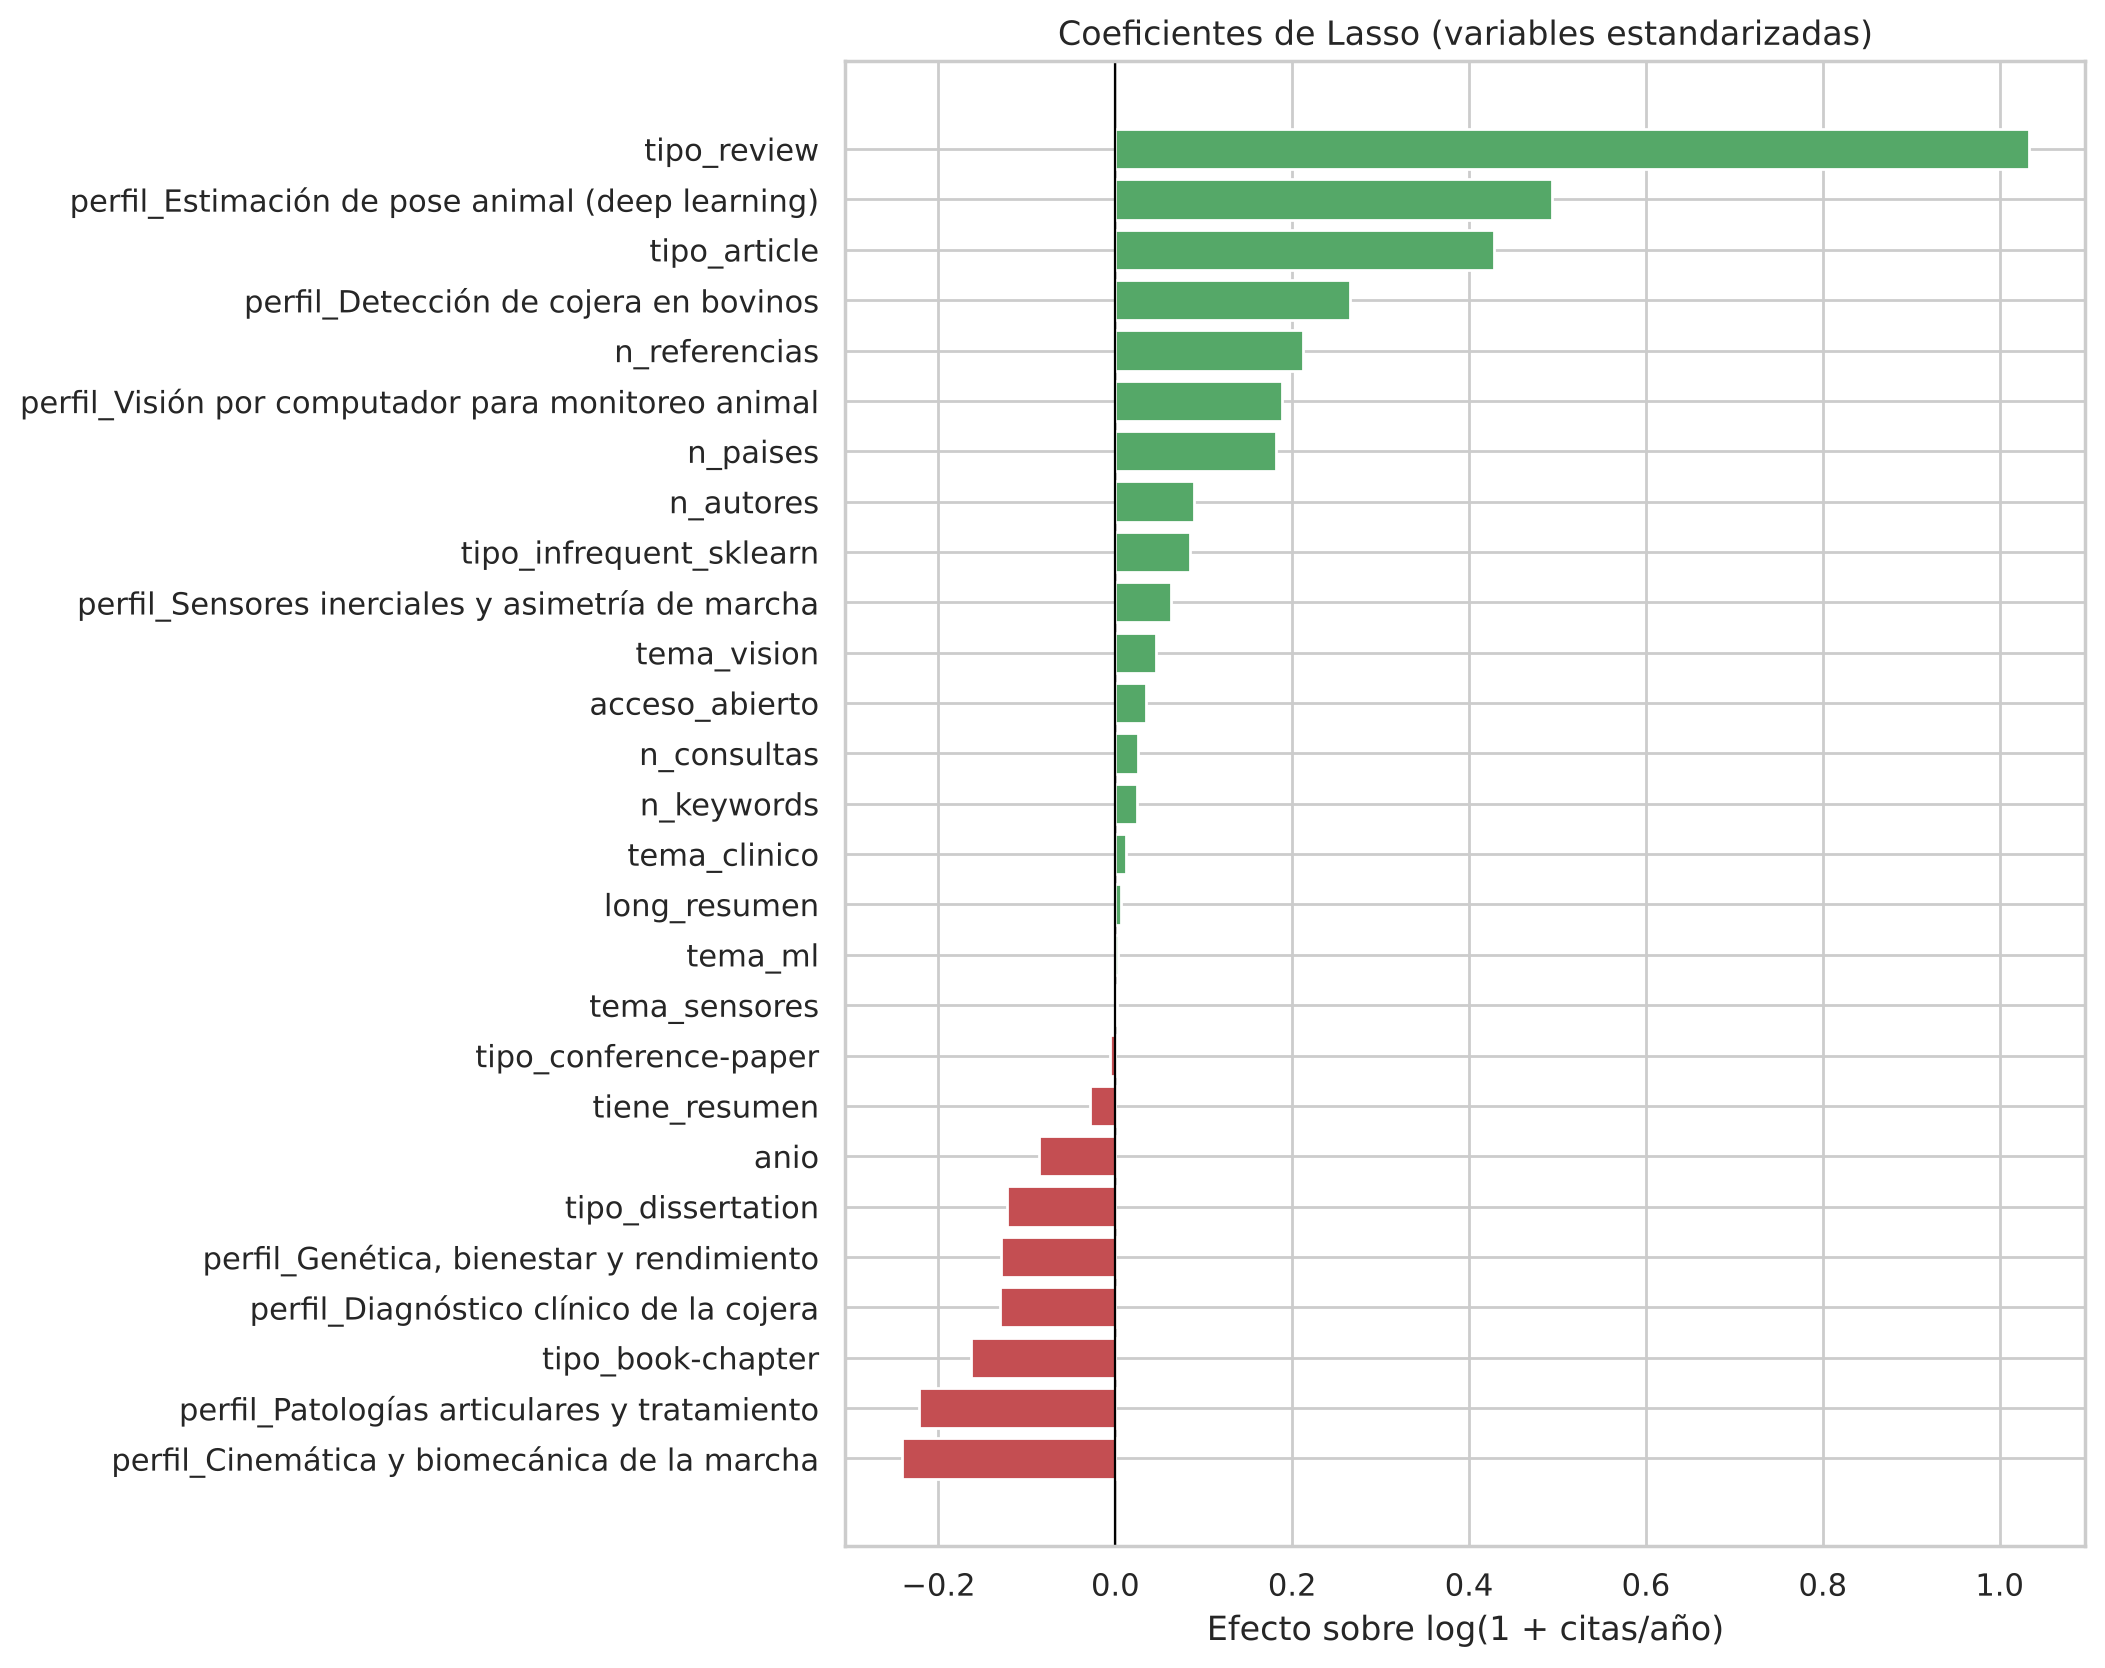
\includegraphics[width=0.9\columnwidth]{reg_lasso_coeficientes.png}
\caption{Coeficientes de Lasso: características asociadas con mayor o menor impacto de un artículo.}
\label{fig:lasso}
\end{figure}

\section{Análisis de costos}

La estimación se hizo con precios de lista de la región us-east-1 para dos escenarios (Tabla II). El escenario académico corresponde al uso actual del proyecto y el piloto proyecta cincuenta clínicas con veinte mil pruebas de trote al mes. El costo académico es prácticamente nulo gracias a un diseño sin servidores. En el piloto el principal peso es el almacenamiento, y la arquitectura escala sin cambios. El costo real, consultado en la consola de facturación de AWS, fue de cero dólares desde el despliegue, porque el uso de estos días quedó cubierto por la capa gratuita de la cuenta, lo que es consistente con la estimación y confirma que la base del sistema puede operar sin costo en un contexto académico.

\begin{table}[!htb]
\centering
\caption{Costo mensual estimado en USD}
\label{tab:costos}
\begin{tabular}{lrr}
\toprule
Servicio & Académico & Piloto \\
\midrule
S3 y réplica de recuperación & 0,17 & 9,80 \\
Lambda y API Gateway & 0,03 & 0,70 \\
DynamoDB y Athena & 0,03 & 1,46 \\
Parameter Store, ECR y CloudWatch & 0,15 & 1,55 \\
\midrule
\textbf{Total sin capa gratuita} & \textbf{0,38} & \textbf{13,51} \\
Total con capa gratuita & 0,13 & 10,95 \\
\bottomrule
\end{tabular}
\end{table}

\section{Discusión}

Los resultados dan respuesta a la pregunta de investigación de manera positiva, aunque mantiene matices. Las medidas de asimetría de la cabeza y la pelvis, que pueden obtenerse con tecnología accesible, bastan para estimar la probabilidad de cojera en caballos que el modelo no conoce. Además, el modelo se apoya en los mismos indicios que la literatura clínica asocia con la cojera anterior y posterior~\cite{keegan2013}, lo que demuestra que aprendió de manera coherente un patrón presente en la naturaleza.

Por otro lado, el desempeño moderado del modelo resultante se debe a que: La cojera inducida fue leve, justo el caso en que los propios veterinarios coinciden poco~\cite{keegan2010,hammarberg2016}, y además algunos caballos demostraron ya ser asimétricos estando sanos, lo que tiende a confundir al umbral general.

La minería del estado del arte y el catálogo de datasets tienen también una implicación práctica: pasar al video exige obtener las mismas trayectorias desde la imagen replicando procesos vistos en los estudios. A la vez, la falta de datos con etiqueta de cojera y de estudios en la región muestra que un aporte local, con caballos criollos, tendría valor científico. En cuanto a la nube, el costo casi nulo indica que la infraestructura no es una barrera para llevar el sistema a un piloto.

\subsection{Limitaciones y trabajo futuro}

Las principales limitaciones son el número reducido de caballos, el uso de cojera inducida y no natural, y una sola raza. El trabajo futuro incluye comparar a cada caballo con su propia línea, así, identificar el lado de la asimetría, estimar un grado de cojera y, en la fase de visión, calcular estas medidas desde video con un modelo de estimación de pose. A más largo plazo, se propone recolectar datos propios de caballos criollos colombianos evaluados por veterinarios, cuyos andares, como el paso fino y la trocha, difieren del trote estudiado en la literatura.

\section{Conclusiones}

La minería de datos fue crucial en esta fase del proyecto ya que permitió mapear un campo que avanza rápido hacia la visión por computador y que deja un vacío claro: no hay datos abiertos de video equino con cojera y casi no hay investigación latinoamericana. Por otra parte, los datos de sensores demostraron una asimetría del movimiento de la cabeza y la pelvis que evidencia la cojera de forma interpretable, y el modelo construido sobre esas medidas funciona con caballos que nunca vio. El sistema completo, desde la ingesta hasta la predicción, quedó desplegado en la nube como código, con un costo casi nulo. Si en la siguiente fase la visión por computador estima esas mismas trayectorias desde un video, el modelo y la infraestructura de este trabajo ya están listos para recibirlas.

\section*{Declaración de uso de inteligencia artificial}

Se utilizó Claude (Anthropic) como herramienta de apoyo en tareas de investigación, organización del documento, revisión de redacción y depuración de código. El autor revisó todo el material y es responsable de su contenido.

\section*{Ética y datos}

Se usaron únicamente datos públicos con licencia abierta y no se trataron datos personales. El protocolo experimental del dataset de sensores es responsabilidad de sus autores. El sistema es una herramienta de apoyo y no reemplaza el examen veterinario.

\begin{thebibliography}{99}
\bibitem{nehs2013} ``Equine health survey highlights the prevalence of lameness,'' \emph{Veterinary Record}, vol.~173, no.~6, p.~132, 2013, doi: 10.1136/vr.f4967.
\bibitem{usda1998} USDA APHIS, ``National economic cost of equine lameness, colic, and equine protozoal myeloencephalitis (EPM) in the United States,'' Info sheet, NAHMS Equine'98, Fort Collins, CO, EE.~UU.
\bibitem{keegan2010} K.~G. Keegan \emph{et al.}, ``Repeatability of subjective evaluation of lameness in horses,'' \emph{Equine Vet. J.}, vol.~42, no.~2, pp.~92--97, 2010, doi: 10.2746/042516409X479568.
\bibitem{hammarberg2016} M.~Hammarberg, A.~Egenvall, T.~Pfau y M.~Rhodin, ``Rater agreement of visual lameness assessment in horses during lungeing,'' \emph{Equine Vet. J.}, vol.~48, no.~1, pp.~78--82, 2016, doi: 10.1111/evj.12385.
\bibitem{agronegocios2025censo} Agronegocios, ``¿Cuántos caballos hay en Colombia y de esta cifra cuántos están registrados?,'' 2025. [En línea]. Disponible: \url{https://www.agronegocios.co/finca/cuantos-caballos-hay-en-colombia-y-de-esta-cifra-cuantos-estan-registrados-4206155}
\bibitem{un2015} Naciones Unidas, ``Transformar nuestro mundo: la Agenda 2030 para el Desarrollo Sostenible,'' Res. A/RES/70/1, 2015.
\bibitem{keegan2013} K.~G. Keegan \emph{et al.}, ``Comparison of a body-mounted inertial sensor system-based method with subjective evaluation for detection of lameness in horses,'' \emph{Am. J. Vet. Res.}, vol.~74, no.~1, pp.~17--24, 2013.
\bibitem{mathis2018} A.~Mathis \emph{et al.}, ``DeepLabCut: markerless pose estimation of user-defined body parts with deep learning,'' \emph{Nature Neuroscience}, vol.~21, pp.~1281--1289, 2018.
\bibitem{mathis2021} A.~Mathis \emph{et al.}, ``Pretraining boosts out-of-domain robustness for pose estimation,'' en \emph{Proc. IEEE/CVF WACV}, 2021, pp.~1859--1868.
\bibitem{li2024pferd} C.~Li \emph{et al.}, ``The Poses for Equine Research Dataset (PFERD),'' \emph{Scientific Data}, vol.~11, art.~497, 2024.
\bibitem{yu2021ap10k} H.~Yu \emph{et al.}, ``AP-10K: A benchmark for animal pose estimation in the wild,'' en \emph{NeurIPS Datasets and Benchmarks Track}, 2021.
\bibitem{yang2022apt36k} Y.~Yang \emph{et al.}, ``APT-36K: A large-scale benchmark for animal pose estimation and tracking,'' en \emph{NeurIPS Datasets and Benchmarks Track}, 2022.
\bibitem{ng2022animalkingdom} X.~L. Ng \emph{et al.}, ``Animal Kingdom: A large and diverse dataset for animal behavior understanding,'' en \emph{Proc. IEEE/CVF CVPR}, 2022, pp.~19023--19034.
\bibitem{ismail2024cow} S.~Ismail \emph{et al.}, ``CowScreeningDB: A public benchmark database for lameness detection in dairy cows,'' \emph{Comput. Electron. Agric.}, vol.~216, art.~108500, 2024.
\bibitem{wirth2000} R.~Wirth y J.~Hipp, ``CRISP-DM: Towards a standard process model for data mining,'' en \emph{Proc. 4th Int. Conf. Practical Applications of Knowledge Discovery and Data Mining}, 2000, pp.~29--39.
\bibitem{agrawal1994} R.~Agrawal y R.~Srikant, ``Fast algorithms for mining association rules,'' en \emph{Proc. 20th Int. Conf. Very Large Data Bases}, 1994, pp.~487--499.
\bibitem{han2000} J.~Han, J.~Pei y Y.~Yin, ``Mining frequent patterns without candidate generation,'' en \emph{Proc. ACM SIGMOD}, 2000, pp.~1--12.
\bibitem{salton1988} G. Salton y C. Buckley, ``Term-weighting approaches in automatic text retrieval,'' \emph{Information Processing \& Management}, vol. 24, no. 5, pp. 513--523, 1988.
\bibitem{lloyd1982} S. Lloyd, ``Least squares quantization in PCM,'' \emph{IEEE Trans. Inf. Theory}, vol. 28, no. 2, pp. 129--137, 1982.
\bibitem{gower1971} J. C. Gower, ``A general coefficient of similarity and some of its properties,'' \emph{Biometrics}, vol. 27, no. 4, pp. 857--871, 1971.
\bibitem{liu2008} F. T. Liu, K. M. Ting y Z.-H. Zhou, ``Isolation forest,'' en \emph{Proc. IEEE Int. Conf. Data Mining (ICDM)}, 2008, pp. 413--422.
\bibitem{breiman2001} L.~Breiman, ``Random forests,'' \emph{Machine Learning}, vol.~45, no.~1, pp.~5--32, 2001.
\bibitem{friedman2001} J. H. Friedman, ``Greedy function approximation: A gradient boosting machine,'' \emph{Annals of Statistics}, vol. 29, no. 5, pp. 1189--1232, 2001.
\bibitem{lundberg2017} S.~M. Lundberg y S.-I. Lee, ``A unified approach to interpreting model predictions,'' en \emph{Advances in Neural Information Processing Systems 30}, 2017, pp.~4765--4774.
\bibitem{zou2005} H.~Zou y T.~Hastie, ``Regularization and variable selection via the elastic net,'' \emph{J. Royal Statistical Society: Series B}, vol.~67, no.~2, pp.~301--320, 2005.
\bibitem{tibshirani1996} R.~Tibshirani, ``Regression shrinkage and selection via the lasso,'' \emph{J. Royal Statistical Society: Series B}, vol.~58, no.~1, pp.~267--288, 1996.
\bibitem{mell2011} P. Mell y T. Grance, ``The NIST definition of cloud computing,'' NIST Special Publication 800-145, 2011.
\bibitem{terraform} HashiCorp, ``Terraform documentation,'' 2026. [En línea]. Disponible: \url{https://developer.hashicorp.com/terraform/docs}
\bibitem{priem2022openalex} J.~Priem, H.~Piwowar y R.~Orr, ``OpenAlex: A fully-open index of scholarly works, authors, venues, institutions, and concepts,'' arXiv:2205.01833, 2022.
\bibitem{smit2023dataset} I.~Smit \emph{et al.}, ``Kinematic data of the Icelandic horse with induced lameness at walk, trot and tölt,'' DataverseNL, 2025, doi: 10.34894/PEWAK6.
\end{thebibliography}

\end{document}
